\documentclass[twoside]{book}

% Packages required by doxygen
\usepackage{calc}
\usepackage{doxygen}
\usepackage{graphicx}
\usepackage[utf8]{inputenc}
\usepackage{makeidx}
\usepackage{multicol}
\usepackage{multirow}
\usepackage{textcomp}
\usepackage[table]{xcolor}

% Font selection
\usepackage[T1]{fontenc}
\usepackage{mathptmx}
\usepackage[scaled=.90]{helvet}
\usepackage{courier}
\usepackage{amssymb}
\usepackage{sectsty}
\renewcommand{\familydefault}{\sfdefault}
\allsectionsfont{%
  \fontseries{bc}\selectfont%
  \color{darkgray}%
}
\renewcommand{\DoxyLabelFont}{%
  \fontseries{bc}\selectfont%
  \color{darkgray}%
}

% Page & text layout
\usepackage{geometry}
\geometry{%
  a4paper,%
  top=2.5cm,%
  bottom=2.5cm,%
  left=2.5cm,%
  right=2.5cm%
}
\tolerance=750
\hfuzz=15pt
\hbadness=750
\setlength{\emergencystretch}{15pt}
\setlength{\parindent}{0cm}
\setlength{\parskip}{0.2cm}
\makeatletter
\renewcommand{\paragraph}{%
  \@startsection{paragraph}{4}{0ex}{-1.0ex}{1.0ex}{%
    \normalfont\normalsize\bfseries\SS@parafont%
  }%
}
\renewcommand{\subparagraph}{%
  \@startsection{subparagraph}{5}{0ex}{-1.0ex}{1.0ex}{%
    \normalfont\normalsize\bfseries\SS@subparafont%
  }%
}
\makeatother

% Headers & footers
\usepackage{fancyhdr}
\pagestyle{fancyplain}
\fancyhead[LE]{\fancyplain{}{\bfseries\thepage}}
\fancyhead[CE]{\fancyplain{}{}}
\fancyhead[RE]{\fancyplain{}{\bfseries\leftmark}}
\fancyhead[LO]{\fancyplain{}{\bfseries\rightmark}}
\fancyhead[CO]{\fancyplain{}{}}
\fancyhead[RO]{\fancyplain{}{\bfseries\thepage}}
\fancyfoot[LE]{\fancyplain{}{}}
\fancyfoot[CE]{\fancyplain{}{}}
\fancyfoot[RE]{\fancyplain{}{\bfseries\scriptsize Generated on Sat Jun 21 2014 14:49:58 for PMIG by Doxygen }}
\fancyfoot[LO]{\fancyplain{}{\bfseries\scriptsize Generated on Sat Jun 21 2014 14:49:58 for PMIG by Doxygen }}
\fancyfoot[CO]{\fancyplain{}{}}
\fancyfoot[RO]{\fancyplain{}{}}
\renewcommand{\footrulewidth}{0.4pt}
\renewcommand{\chaptermark}[1]{%
  \markboth{#1}{}%
}
\renewcommand{\sectionmark}[1]{%
  \markright{\thesection\ #1}%
}

% Indices & bibliography
\usepackage{natbib}
\usepackage[titles]{tocloft}
\setcounter{tocdepth}{3}
\setcounter{secnumdepth}{5}
\makeindex

% Hyperlinks (required, but should be loaded last)
\usepackage{ifpdf}
\ifpdf
  \usepackage[pdftex,pagebackref=true]{hyperref}
\else
  \usepackage[ps2pdf,pagebackref=true]{hyperref}
\fi
\hypersetup{%
  colorlinks=true,%
  linkcolor=blue,%
  citecolor=blue,%
  unicode%
}

% Custom commands
\newcommand{\clearemptydoublepage}{%
  \newpage{\pagestyle{empty}\cleardoublepage}%
}


%===== C O N T E N T S =====

\begin{document}

% Titlepage & ToC
\hypersetup{pageanchor=false}
\pagenumbering{roman}
\begin{titlepage}
\vspace*{7cm}
\begin{center}%
{\Large P\-M\-I\-G \\[1ex]\large 0.\-6 }\\
\vspace*{1cm}
{\large Generated by Doxygen 1.8.4}\\
\vspace*{0.5cm}
{\small Sat Jun 21 2014 14:49:58}\\
\end{center}
\end{titlepage}
\clearemptydoublepage
\tableofcontents
\clearemptydoublepage
\pagenumbering{arabic}
\hypersetup{pageanchor=true}

%--- Begin generated contents ---
\chapter{\#P\-M\-I\-G}
\label{md_README}
\hypertarget{md_README}{}
\subsubsection*{Summary}

P\-M\-I\-G is a simple image processing tool. The name P\-M\-I\-G is just a tricky reverse of the powerful open software G\-I\-M\-P. \subsubsection*{Platform}

cross \subsubsection*{Development Platform}

xubuntu 13.\-10 \subsubsection*{Kit}

qt designer \subsubsection*{Lang}

c++ \subsubsection*{3rd-\/party lib}

qt5 opencv 2.\-4.\-9 
\chapter{Hierarchical Index}
\section{Class Hierarchy}
This inheritance list is sorted roughly, but not completely, alphabetically\-:\begin{DoxyCompactList}
\item \contentsline{section}{Brush\-Tool\-Base}{\pageref{class_brush_tool_base}}{}
\begin{DoxyCompactList}
\item \contentsline{section}{Brush\-Tool\-Function}{\pageref{class_brush_tool_function}}{}
\item \contentsline{section}{Brush\-Tool\-Tweak}{\pageref{class_brush_tool_tweak}}{}
\end{DoxyCompactList}
\item \contentsline{section}{Erase\-Tool\-Base}{\pageref{class_erase_tool_base}}{}
\begin{DoxyCompactList}
\item \contentsline{section}{Erase\-Tool\-Function}{\pageref{class_erase_tool_function}}{}
\item \contentsline{section}{Erase\-Tool\-Tweak}{\pageref{class_erase_tool_tweak}}{}
\end{DoxyCompactList}
\item \contentsline{section}{Lasso\-Tool\-Base}{\pageref{class_lasso_tool_base}}{}
\begin{DoxyCompactList}
\item \contentsline{section}{Lasso\-Tool\-Function}{\pageref{class_lasso_tool_function}}{}
\item \contentsline{section}{Lasso\-Tool\-Tweak}{\pageref{class_lasso_tool_tweak}}{}
\end{DoxyCompactList}
\item \contentsline{section}{Layer}{\pageref{struct_layer}}{}
\item \contentsline{section}{Marquee\-Tool\-Base}{\pageref{class_marquee_tool_base}}{}
\begin{DoxyCompactList}
\item \contentsline{section}{Marquee\-Tool\-Function}{\pageref{class_marquee_tool_function}}{}
\item \contentsline{section}{Marquee\-Tool\-Tweak}{\pageref{class_marquee_tool_tweak}}{}
\end{DoxyCompactList}
\item \contentsline{section}{Pen\-Tool\-Base}{\pageref{class_pen_tool_base}}{}
\begin{DoxyCompactList}
\item \contentsline{section}{Pen\-Tool\-Function}{\pageref{class_pen_tool_function}}{}
\item \contentsline{section}{Pen\-Tool\-Tweak}{\pageref{class_pen_tool_tweak}}{}
\end{DoxyCompactList}
\item Q\-Action\begin{DoxyCompactList}
\item \contentsline{section}{Color\-Icon\-Action}{\pageref{class_color_icon_action}}{}
\end{DoxyCompactList}
\item Q\-Dock\-Widget\begin{DoxyCompactList}
\item \contentsline{section}{Color\-Swatch}{\pageref{class_color_swatch}}{}
\end{DoxyCompactList}
\item Q\-Frame\begin{DoxyCompactList}
\item \contentsline{section}{Color\-Dock}{\pageref{class_color_dock}}{}
\end{DoxyCompactList}
\item Q\-Main\-Window\begin{DoxyCompactList}
\item \contentsline{section}{Main\-Window}{\pageref{class_main_window}}{}
\end{DoxyCompactList}
\item Q\-Object\begin{DoxyCompactList}
\item \contentsline{section}{Brush\-Tool\-Function}{\pageref{class_brush_tool_function}}{}
\item \contentsline{section}{Erase\-Tool\-Function}{\pageref{class_erase_tool_function}}{}
\item \contentsline{section}{Lasso\-Tool\-Function}{\pageref{class_lasso_tool_function}}{}
\item \contentsline{section}{Marquee\-Tool\-Function}{\pageref{class_marquee_tool_function}}{}
\item \contentsline{section}{Pen\-Tool\-Function}{\pageref{class_pen_tool_function}}{}
\item \contentsline{section}{Tool\-Box}{\pageref{class_tool_box}}{}
\item \contentsline{section}{Transform\-Tool\-Function}{\pageref{class_transform_tool_function}}{}
\end{DoxyCompactList}
\item Q\-Stack\begin{DoxyCompactList}
\item \contentsline{section}{Layer\-Stack}{\pageref{class_layer_stack}}{}
\end{DoxyCompactList}
\item Q\-Tool\-Bar\begin{DoxyCompactList}
\item \contentsline{section}{Tool\-Bar}{\pageref{class_tool_bar}}{}
\item \contentsline{section}{Tool\-Tweak}{\pageref{class_tool_tweak}}{}
\begin{DoxyCompactList}
\item \contentsline{section}{Brush\-Tool\-Tweak}{\pageref{class_brush_tool_tweak}}{}
\item \contentsline{section}{Erase\-Tool\-Tweak}{\pageref{class_erase_tool_tweak}}{}
\item \contentsline{section}{Lasso\-Tool\-Tweak}{\pageref{class_lasso_tool_tweak}}{}
\item \contentsline{section}{Marquee\-Tool\-Tweak}{\pageref{class_marquee_tool_tweak}}{}
\item \contentsline{section}{Pen\-Tool\-Tweak}{\pageref{class_pen_tool_tweak}}{}
\item \contentsline{section}{Transform\-Tool\-Tweak}{\pageref{class_transform_tool_tweak}}{}
\end{DoxyCompactList}
\end{DoxyCompactList}
\item Q\-Widget\begin{DoxyCompactList}
\item \contentsline{section}{Blue\-Title\-Bar}{\pageref{class_blue_title_bar}}{}
\item \contentsline{section}{Scribble\-Area}{\pageref{class_scribble_area}}{}
\end{DoxyCompactList}
\item \contentsline{section}{Tool\-Type}{\pageref{class_tool_type}}{}
\item \contentsline{section}{Transform\-Tool\-Base}{\pageref{class_transform_tool_base}}{}
\begin{DoxyCompactList}
\item \contentsline{section}{Transform\-Tool\-Function}{\pageref{class_transform_tool_function}}{}
\item \contentsline{section}{Transform\-Tool\-Tweak}{\pageref{class_transform_tool_tweak}}{}
\end{DoxyCompactList}
\end{DoxyCompactList}

\chapter{Class Index}
\section{Class List}
Here are the classes, structs, unions and interfaces with brief descriptions\-:\begin{DoxyCompactList}
\item\contentsline{section}{\hyperlink{class_blue_title_bar}{Blue\-Title\-Bar} }{\pageref{class_blue_title_bar}}{}
\item\contentsline{section}{\hyperlink{class_brush_tool_base}{Brush\-Tool\-Base} }{\pageref{class_brush_tool_base}}{}
\item\contentsline{section}{\hyperlink{class_brush_tool_function}{Brush\-Tool\-Function} }{\pageref{class_brush_tool_function}}{}
\item\contentsline{section}{\hyperlink{class_brush_tool_tweak}{Brush\-Tool\-Tweak} }{\pageref{class_brush_tool_tweak}}{}
\item\contentsline{section}{\hyperlink{class_color_dock}{Color\-Dock} }{\pageref{class_color_dock}}{}
\item\contentsline{section}{\hyperlink{class_color_icon_action}{Color\-Icon\-Action} }{\pageref{class_color_icon_action}}{}
\item\contentsline{section}{\hyperlink{class_color_swatch}{Color\-Swatch} }{\pageref{class_color_swatch}}{}
\item\contentsline{section}{\hyperlink{class_erase_tool_base}{Erase\-Tool\-Base} }{\pageref{class_erase_tool_base}}{}
\item\contentsline{section}{\hyperlink{class_erase_tool_function}{Erase\-Tool\-Function} }{\pageref{class_erase_tool_function}}{}
\item\contentsline{section}{\hyperlink{class_erase_tool_tweak}{Erase\-Tool\-Tweak} }{\pageref{class_erase_tool_tweak}}{}
\item\contentsline{section}{\hyperlink{class_lasso_tool_base}{Lasso\-Tool\-Base} }{\pageref{class_lasso_tool_base}}{}
\item\contentsline{section}{\hyperlink{class_lasso_tool_function}{Lasso\-Tool\-Function} }{\pageref{class_lasso_tool_function}}{}
\item\contentsline{section}{\hyperlink{class_lasso_tool_tweak}{Lasso\-Tool\-Tweak} }{\pageref{class_lasso_tool_tweak}}{}
\item\contentsline{section}{\hyperlink{struct_layer}{Layer} }{\pageref{struct_layer}}{}
\item\contentsline{section}{\hyperlink{class_layer_stack}{Layer\-Stack} }{\pageref{class_layer_stack}}{}
\item\contentsline{section}{\hyperlink{class_main_window}{Main\-Window} \\*Create a \hyperlink{class_main_window}{Main\-Window} }{\pageref{class_main_window}}{}
\item\contentsline{section}{\hyperlink{class_marquee_tool_base}{Marquee\-Tool\-Base} }{\pageref{class_marquee_tool_base}}{}
\item\contentsline{section}{\hyperlink{class_marquee_tool_function}{Marquee\-Tool\-Function} }{\pageref{class_marquee_tool_function}}{}
\item\contentsline{section}{\hyperlink{class_marquee_tool_tweak}{Marquee\-Tool\-Tweak} }{\pageref{class_marquee_tool_tweak}}{}
\item\contentsline{section}{\hyperlink{class_pen_tool_base}{Pen\-Tool\-Base} }{\pageref{class_pen_tool_base}}{}
\item\contentsline{section}{\hyperlink{class_pen_tool_function}{Pen\-Tool\-Function} }{\pageref{class_pen_tool_function}}{}
\item\contentsline{section}{\hyperlink{class_pen_tool_tweak}{Pen\-Tool\-Tweak} }{\pageref{class_pen_tool_tweak}}{}
\item\contentsline{section}{\hyperlink{class_scribble_area}{Scribble\-Area} \\*\mbox{[}0\mbox{]} }{\pageref{class_scribble_area}}{}
\item\contentsline{section}{\hyperlink{class_tool_bar}{Tool\-Bar} }{\pageref{class_tool_bar}}{}
\item\contentsline{section}{\hyperlink{class_tool_box}{Tool\-Box} }{\pageref{class_tool_box}}{}
\item\contentsline{section}{\hyperlink{class_tool_tweak}{Tool\-Tweak} }{\pageref{class_tool_tweak}}{}
\item\contentsline{section}{\hyperlink{class_tool_type}{Tool\-Type} }{\pageref{class_tool_type}}{}
\item\contentsline{section}{\hyperlink{class_transform_tool_base}{Transform\-Tool\-Base} }{\pageref{class_transform_tool_base}}{}
\item\contentsline{section}{\hyperlink{class_transform_tool_function}{Transform\-Tool\-Function} }{\pageref{class_transform_tool_function}}{}
\item\contentsline{section}{\hyperlink{class_transform_tool_tweak}{Transform\-Tool\-Tweak} }{\pageref{class_transform_tool_tweak}}{}
\end{DoxyCompactList}

\chapter{Class Documentation}
\hypertarget{class_blue_title_bar}{\section{Blue\-Title\-Bar Class Reference}
\label{class_blue_title_bar}\index{Blue\-Title\-Bar@{Blue\-Title\-Bar}}
}
Inheritance diagram for Blue\-Title\-Bar\-:\begin{figure}[H]
\begin{center}
\leavevmode
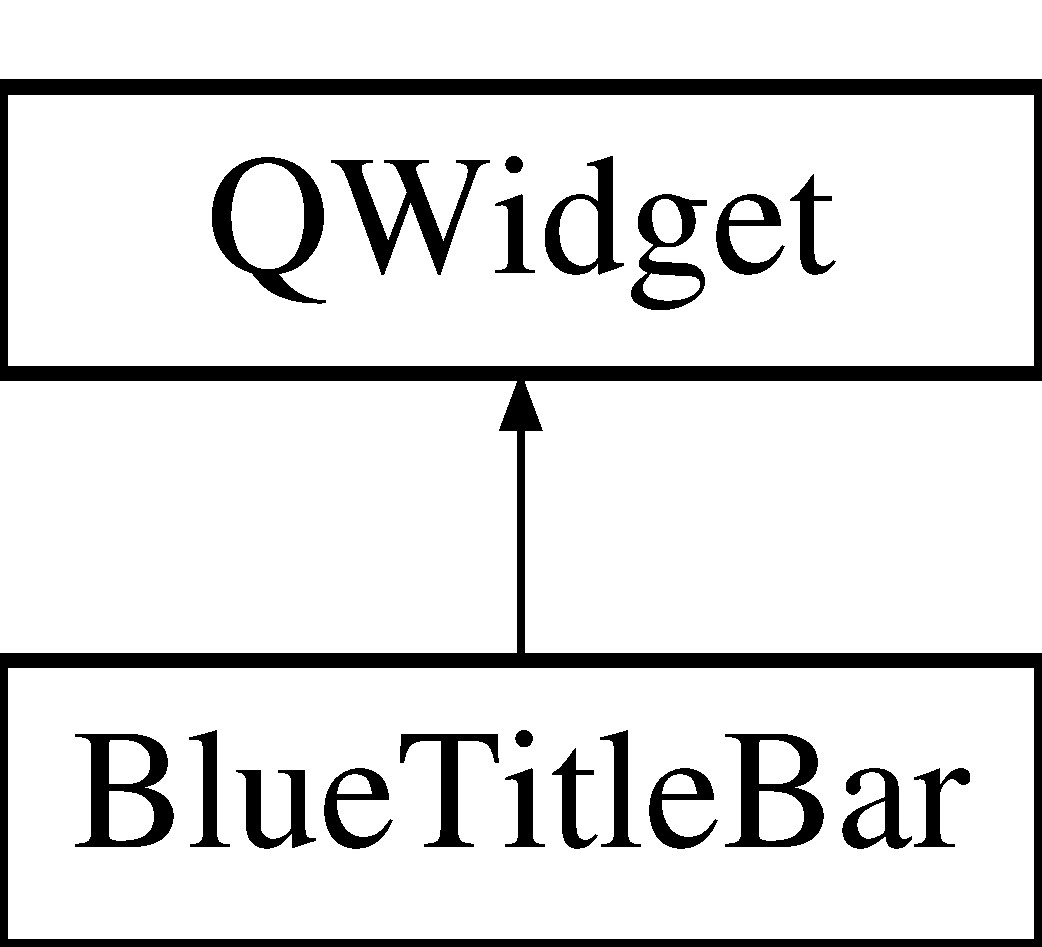
\includegraphics[height=2.000000cm]{class_blue_title_bar}
\end{center}
\end{figure}
\subsection*{Public Slots}
\begin{DoxyCompactItemize}
\item 
void \hyperlink{class_blue_title_bar_abdf4de317ce7595d8915607c4dacce44}{update\-Mask} ()
\end{DoxyCompactItemize}
\subsection*{Public Member Functions}
\begin{DoxyCompactItemize}
\item 
\hypertarget{class_blue_title_bar_ab04ab26d6f841529aa35eb04d34345ec}{{\bfseries Blue\-Title\-Bar} (Q\-Widget $\ast$parent=0)}\label{class_blue_title_bar_ab04ab26d6f841529aa35eb04d34345ec}

\item 
\hypertarget{class_blue_title_bar_a42d8bca94135de0f79e9a213fb385b44}{Q\-Size {\bfseries size\-Hint} () const }\label{class_blue_title_bar_a42d8bca94135de0f79e9a213fb385b44}

\item 
\hypertarget{class_blue_title_bar_a6212f3c1bd29270b250e7a8b83af360c}{Q\-Size {\bfseries minimum\-Size\-Hint} () const }\label{class_blue_title_bar_a6212f3c1bd29270b250e7a8b83af360c}

\end{DoxyCompactItemize}
\subsection*{Protected Member Functions}
\begin{DoxyCompactItemize}
\item 
\hypertarget{class_blue_title_bar_a522509f27521585391c8678a7cfb9868}{void {\bfseries paint\-Event} (Q\-Paint\-Event $\ast$event)}\label{class_blue_title_bar_a522509f27521585391c8678a7cfb9868}

\item 
\hypertarget{class_blue_title_bar_ac3867646e0062f145fdd25747bcad614}{void {\bfseries mouse\-Press\-Event} (Q\-Mouse\-Event $\ast$event)}\label{class_blue_title_bar_ac3867646e0062f145fdd25747bcad614}

\end{DoxyCompactItemize}


\subsection{Member Function Documentation}
\hypertarget{class_blue_title_bar_abdf4de317ce7595d8915607c4dacce44}{\index{Blue\-Title\-Bar@{Blue\-Title\-Bar}!update\-Mask@{update\-Mask}}
\index{update\-Mask@{update\-Mask}!BlueTitleBar@{Blue\-Title\-Bar}}
\subsubsection[{update\-Mask}]{\setlength{\rightskip}{0pt plus 5cm}void Blue\-Title\-Bar\-::update\-Mask (
\begin{DoxyParamCaption}
{}
\end{DoxyParamCaption}
)\hspace{0.3cm}{\ttfamily [slot]}}}\label{class_blue_title_bar_abdf4de317ce7595d8915607c4dacce44}
initialize to transparent 

The documentation for this class was generated from the following files\-:\begin{DoxyCompactItemize}
\item 
colorswatch.\-h\item 
colorswatch.\-cpp\end{DoxyCompactItemize}

\hypertarget{class_brush_tool_base}{\section{Brush\-Tool\-Base Class Reference}
\label{class_brush_tool_base}\index{Brush\-Tool\-Base@{Brush\-Tool\-Base}}
}
Inheritance diagram for Brush\-Tool\-Base\-:\begin{figure}[H]
\begin{center}
\leavevmode
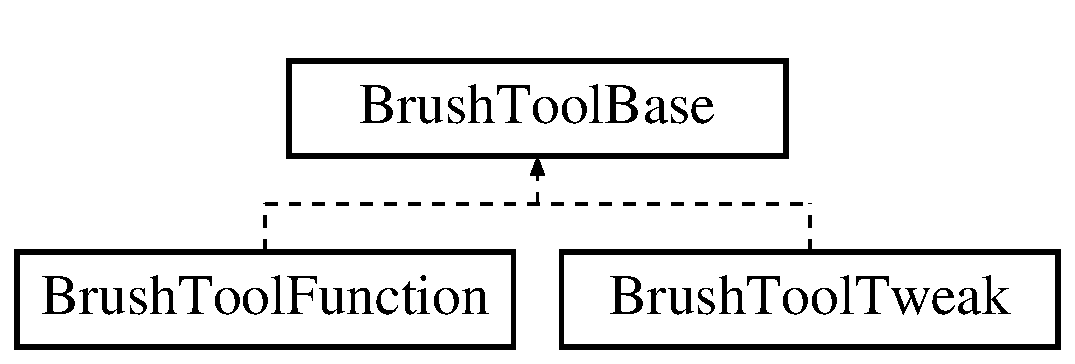
\includegraphics[height=2.000000cm]{class_brush_tool_base}
\end{center}
\end{figure}
\subsection*{Static Protected Attributes}
\begin{DoxyCompactItemize}
\item 
\hypertarget{class_brush_tool_base_aa6fa9de97a6648fe8780a67ed73389da}{static int {\bfseries brush\-Size} =2}\label{class_brush_tool_base_aa6fa9de97a6648fe8780a67ed73389da}

\item 
\hypertarget{class_brush_tool_base_a945641cf5a7298842c2f43972688ab10}{static int {\bfseries line\-Type}}\label{class_brush_tool_base_a945641cf5a7298842c2f43972688ab10}

\item 
\hypertarget{class_brush_tool_base_aa420951020c02551baf64d01ade5d33c}{static bool {\bfseries anti\-Aliasing}}\label{class_brush_tool_base_aa420951020c02551baf64d01ade5d33c}

\end{DoxyCompactItemize}


The documentation for this class was generated from the following files\-:\begin{DoxyCompactItemize}
\item 
toolbox.\-h\item 
toolbox.\-cpp\end{DoxyCompactItemize}

\hypertarget{class_brush_tool_function}{\section{Brush\-Tool\-Function Class Reference}
\label{class_brush_tool_function}\index{Brush\-Tool\-Function@{Brush\-Tool\-Function}}
}
Inheritance diagram for Brush\-Tool\-Function\-:\begin{figure}[H]
\begin{center}
\leavevmode
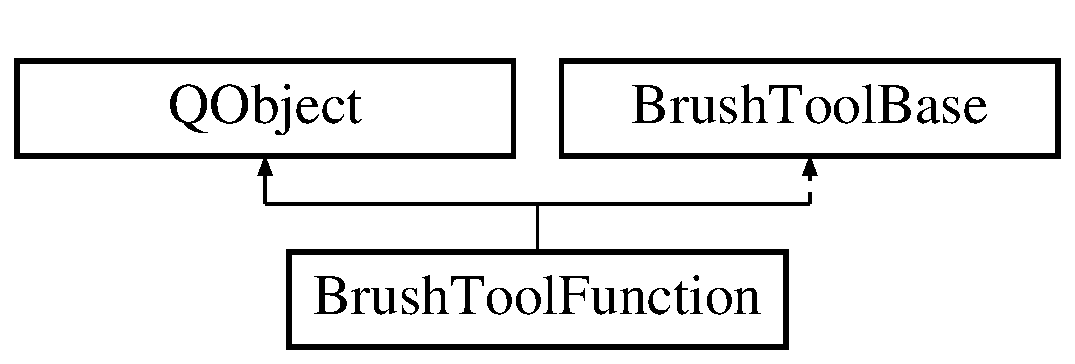
\includegraphics[height=2.000000cm]{class_brush_tool_function}
\end{center}
\end{figure}
\subsection*{Public Member Functions}
\begin{DoxyCompactItemize}
\item 
\hypertarget{class_brush_tool_function_aa1cb6986ab30ae64128002c692d4290f}{{\bfseries Brush\-Tool\-Function} (Q\-Widget $\ast$parent)}\label{class_brush_tool_function_aa1cb6986ab30ae64128002c692d4290f}

\item 
\hypertarget{class_brush_tool_function_a827a6a848f2246a63f58f876b950d0cf}{int {\bfseries get\-Brush\-Size} () const }\label{class_brush_tool_function_a827a6a848f2246a63f58f876b950d0cf}

\item 
\hypertarget{class_brush_tool_function_a49319b286a0b4a9f7e093963ac123b26}{int {\bfseries get\-Line\-Type} () const }\label{class_brush_tool_function_a49319b286a0b4a9f7e093963ac123b26}

\item 
\hypertarget{class_brush_tool_function_a0665bc3c2c304b5889629680912484a5}{bool {\bfseries get\-Anti\-Aliasing} () const }\label{class_brush_tool_function_a0665bc3c2c304b5889629680912484a5}

\end{DoxyCompactItemize}
\subsection*{Additional Inherited Members}


The documentation for this class was generated from the following files\-:\begin{DoxyCompactItemize}
\item 
toolbox.\-h\item 
toolbox.\-cpp\end{DoxyCompactItemize}

\hypertarget{class_brush_tool_tweak}{\section{Brush\-Tool\-Tweak Class Reference}
\label{class_brush_tool_tweak}\index{Brush\-Tool\-Tweak@{Brush\-Tool\-Tweak}}
}
Inheritance diagram for Brush\-Tool\-Tweak\-:\begin{figure}[H]
\begin{center}
\leavevmode
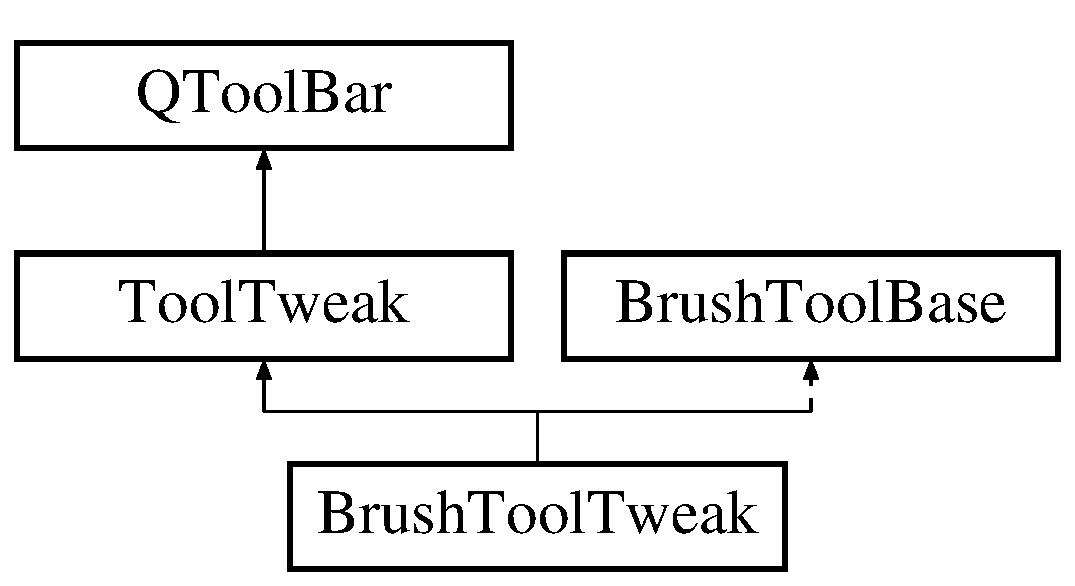
\includegraphics[height=3.000000cm]{class_brush_tool_tweak}
\end{center}
\end{figure}
\subsection*{Public Member Functions}
\begin{DoxyCompactItemize}
\item 
\hypertarget{class_brush_tool_tweak_aeed0fc50628c810b5a01ace5f28d50d7}{{\bfseries Brush\-Tool\-Tweak} (Q\-Widget $\ast$parent)}\label{class_brush_tool_tweak_aeed0fc50628c810b5a01ace5f28d50d7}

\end{DoxyCompactItemize}
\subsection*{Additional Inherited Members}


The documentation for this class was generated from the following files\-:\begin{DoxyCompactItemize}
\item 
toolbox.\-h\item 
toolbox.\-cpp\end{DoxyCompactItemize}

\hypertarget{class_color_dock}{\section{Color\-Dock Class Reference}
\label{class_color_dock}\index{Color\-Dock@{Color\-Dock}}
}
Inheritance diagram for Color\-Dock\-:\begin{figure}[H]
\begin{center}
\leavevmode
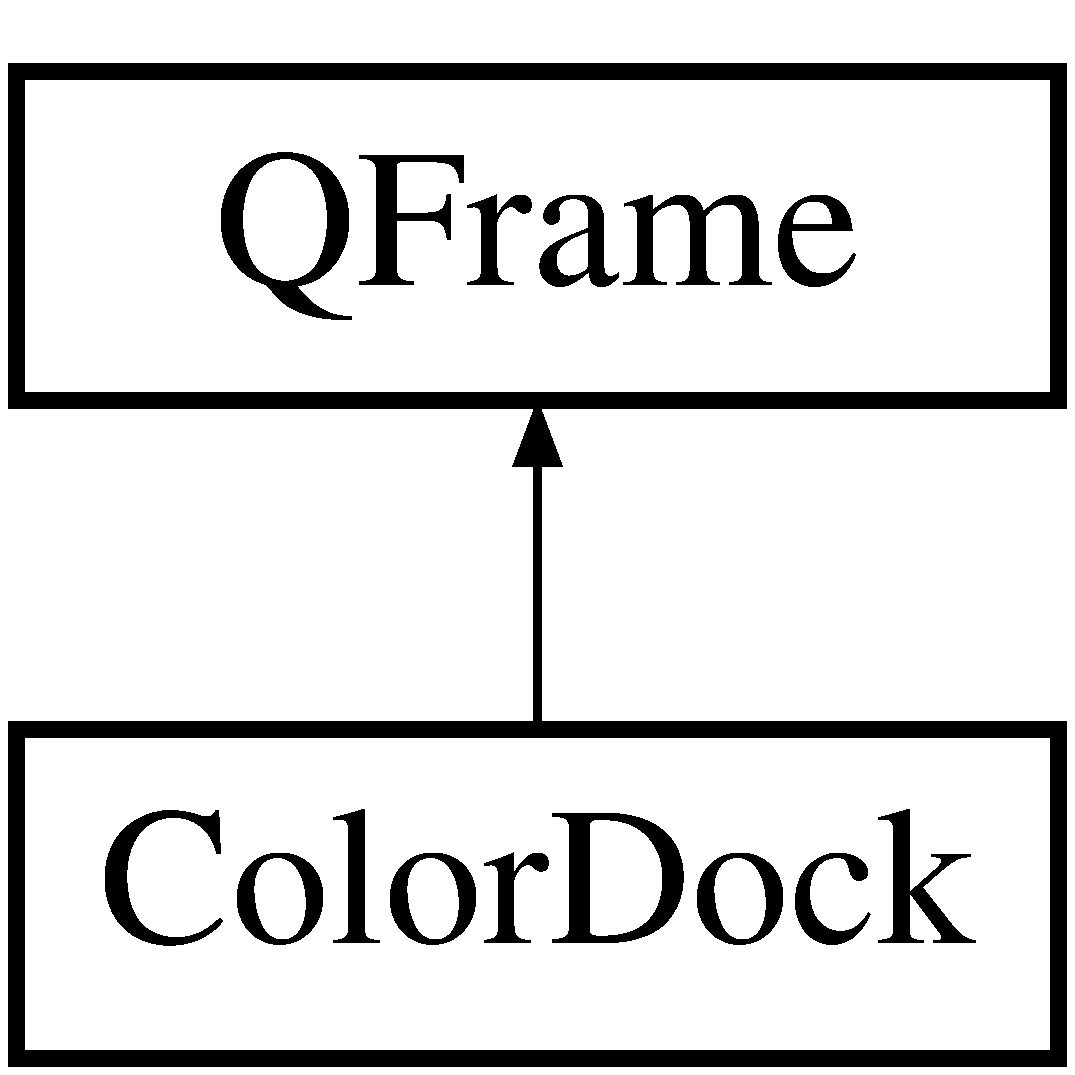
\includegraphics[height=2.000000cm]{class_color_dock}
\end{center}
\end{figure}
\subsection*{Public Slots}
\begin{DoxyCompactItemize}
\item 
\hypertarget{class_color_dock_af2659c6d290c1326e1757a787f047509}{void {\bfseries change\-Size\-Hints} ()}\label{class_color_dock_af2659c6d290c1326e1757a787f047509}

\end{DoxyCompactItemize}
\subsection*{Public Member Functions}
\begin{DoxyCompactItemize}
\item 
\hypertarget{class_color_dock_a178888e49538d53e7c4331ed0c0b4e52}{{\bfseries Color\-Dock} (const Q\-String \&c, Q\-Widget $\ast$parent)}\label{class_color_dock_a178888e49538d53e7c4331ed0c0b4e52}

\item 
\hypertarget{class_color_dock_a116198e960d54f2393f4f1b14a3e2162}{virtual Q\-Size {\bfseries size\-Hint} () const }\label{class_color_dock_a116198e960d54f2393f4f1b14a3e2162}

\item 
\hypertarget{class_color_dock_aef209e5c9adcf99664c07c65633c83e6}{virtual Q\-Size {\bfseries minimum\-Size\-Hint} () const }\label{class_color_dock_aef209e5c9adcf99664c07c65633c83e6}

\item 
\hypertarget{class_color_dock_a94da7c005c8f0454038dd4534cba5a25}{void {\bfseries set\-Custom\-Size\-Hint} (const Q\-Size \&size)}\label{class_color_dock_a94da7c005c8f0454038dd4534cba5a25}

\end{DoxyCompactItemize}
\subsection*{Protected Member Functions}
\begin{DoxyCompactItemize}
\item 
\hypertarget{class_color_dock_af228e7700f3fb422a22770b170a93400}{void {\bfseries paint\-Event} (Q\-Paint\-Event $\ast$)}\label{class_color_dock_af228e7700f3fb422a22770b170a93400}

\end{DoxyCompactItemize}
\subsection*{Protected Attributes}
\begin{DoxyCompactItemize}
\item 
\hypertarget{class_color_dock_aea4e5ea45303ea9b34da836180f6158f}{Q\-String {\bfseries color}}\label{class_color_dock_aea4e5ea45303ea9b34da836180f6158f}

\item 
\hypertarget{class_color_dock_aea0335333213f94689cc827db1a8d43e}{Q\-Size {\bfseries sz\-Hint}}\label{class_color_dock_aea0335333213f94689cc827db1a8d43e}

\item 
\hypertarget{class_color_dock_aaa99d4fc29b1e011fdfdc562f93ffe90}{Q\-Size {\bfseries min\-Sz\-Hint}}\label{class_color_dock_aaa99d4fc29b1e011fdfdc562f93ffe90}

\end{DoxyCompactItemize}


The documentation for this class was generated from the following file\-:\begin{DoxyCompactItemize}
\item 
colorswatch.\-cpp\end{DoxyCompactItemize}

\hypertarget{class_color_icon_action}{\section{Color\-Icon\-Action Class Reference}
\label{class_color_icon_action}\index{Color\-Icon\-Action@{Color\-Icon\-Action}}
}
Inheritance diagram for Color\-Icon\-Action\-:\begin{figure}[H]
\begin{center}
\leavevmode
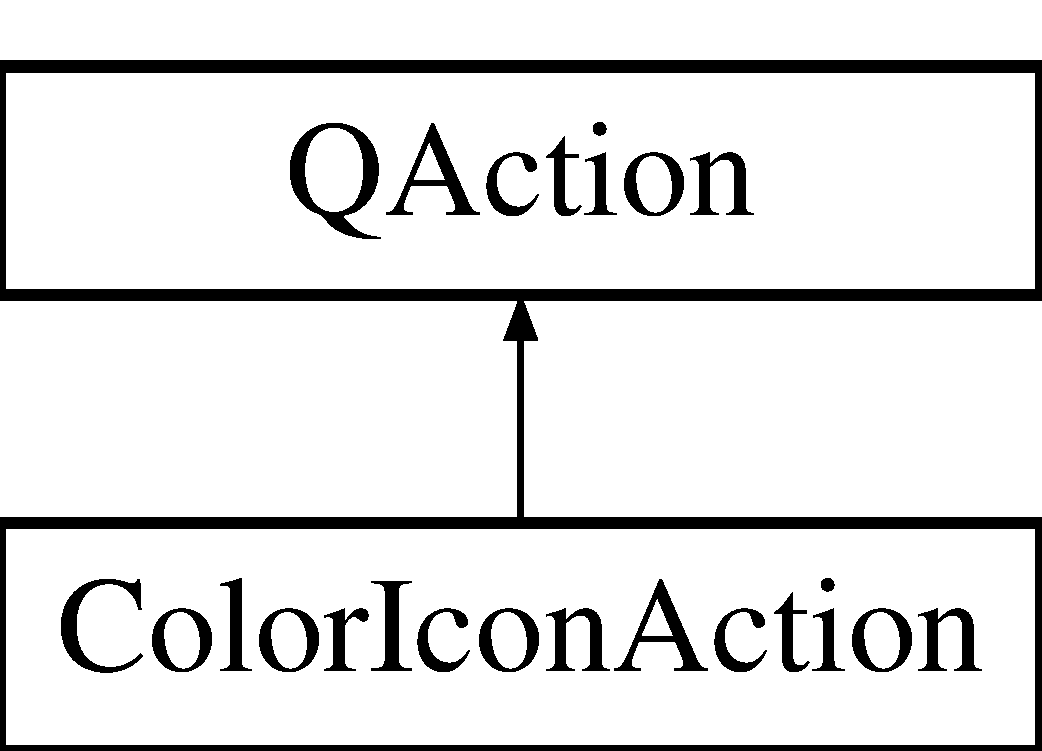
\includegraphics[height=2.000000cm]{class_color_icon_action}
\end{center}
\end{figure}
\subsection*{Public Slots}
\begin{DoxyCompactItemize}
\item 
void \hyperlink{class_color_icon_action_ae1e19112ea77d9b530119ca8f5b9df1b}{update\-Color\-Icon} (int \hyperlink{class_color_icon_action_a11d799bf0358f7a23d4dcf6260612d5c}{id}, Q\-Color color)
\begin{DoxyCompactList}\small\item\em Update the icon of the action when color changes. \end{DoxyCompactList}\end{DoxyCompactItemize}
\subsection*{Public Member Functions}
\begin{DoxyCompactItemize}
\item 
\hyperlink{class_color_icon_action_aabc8d51f340cf2681ada53e6533484fb}{Color\-Icon\-Action} (const Q\-Icon \&icon, const Q\-String \&text, Q\-Object $\ast$parent)
\end{DoxyCompactItemize}
\subsection*{Public Attributes}
\begin{DoxyCompactItemize}
\item 
int \hyperlink{class_color_icon_action_a11d799bf0358f7a23d4dcf6260612d5c}{id}
\end{DoxyCompactItemize}
\subsection*{Static Public Attributes}
\begin{DoxyCompactItemize}
\item 
\hypertarget{class_color_icon_action_af81a6dc58f84719ba6d7f3978e11cf5f}{static int \hyperlink{class_color_icon_action_af81a6dc58f84719ba6d7f3978e11cf5f}{action\-Num}}\label{class_color_icon_action_af81a6dc58f84719ba6d7f3978e11cf5f}

\begin{DoxyCompactList}\small\item\em Static num to track the number of objects have been created. \end{DoxyCompactList}\end{DoxyCompactItemize}


\subsection{Detailed Description}
Used to generate the color button on the toolbox, this action can update icon when necessary 

\subsection{Constructor \& Destructor Documentation}
\hypertarget{class_color_icon_action_aabc8d51f340cf2681ada53e6533484fb}{\index{Color\-Icon\-Action@{Color\-Icon\-Action}!Color\-Icon\-Action@{Color\-Icon\-Action}}
\index{Color\-Icon\-Action@{Color\-Icon\-Action}!ColorIconAction@{Color\-Icon\-Action}}
\subsubsection[{Color\-Icon\-Action}]{\setlength{\rightskip}{0pt plus 5cm}Color\-Icon\-Action\-::\-Color\-Icon\-Action (
\begin{DoxyParamCaption}
\item[{const Q\-Icon \&}]{icon, }
\item[{const Q\-String \&}]{text, }
\item[{Q\-Object $\ast$}]{parent}
\end{DoxyParamCaption}
)\hspace{0.3cm}{\ttfamily [inline]}}}\label{class_color_icon_action_aabc8d51f340cf2681ada53e6533484fb}
Constructor 
\begin{DoxyParams}{Parameters}
{\em \mbox{[}const} & Q\-Icon \&icon\mbox{]} Icon of the action \\
\hline
{\em \mbox{[}const} & Q\-String \&text\mbox{]} Label of the action \\
\hline
{\em \mbox{[}\-Q\-Object} & $\ast$parent\mbox{]} Parent widget. \\
\hline
\end{DoxyParams}


\subsection{Member Function Documentation}
\hypertarget{class_color_icon_action_ae1e19112ea77d9b530119ca8f5b9df1b}{\index{Color\-Icon\-Action@{Color\-Icon\-Action}!update\-Color\-Icon@{update\-Color\-Icon}}
\index{update\-Color\-Icon@{update\-Color\-Icon}!ColorIconAction@{Color\-Icon\-Action}}
\subsubsection[{update\-Color\-Icon}]{\setlength{\rightskip}{0pt plus 5cm}void Color\-Icon\-Action\-::update\-Color\-Icon (
\begin{DoxyParamCaption}
\item[{int}]{id, }
\item[{Q\-Color}]{color}
\end{DoxyParamCaption}
)\hspace{0.3cm}{\ttfamily [slot]}}}\label{class_color_icon_action_ae1e19112ea77d9b530119ca8f5b9df1b}


Update the icon of the action when color changes. 


\begin{DoxyParams}{Parameters}
{\em \mbox{[}int} & id\mbox{]} Indicate which icon to update according to this id \\
\hline
{\em \mbox{[}\-Q\-Color} & color\mbox{]} The new color \\
\hline
\end{DoxyParams}


\subsection{Member Data Documentation}
\hypertarget{class_color_icon_action_a11d799bf0358f7a23d4dcf6260612d5c}{\index{Color\-Icon\-Action@{Color\-Icon\-Action}!id@{id}}
\index{id@{id}!ColorIconAction@{Color\-Icon\-Action}}
\subsubsection[{id}]{\setlength{\rightskip}{0pt plus 5cm}int Color\-Icon\-Action\-::id}}\label{class_color_icon_action_a11d799bf0358f7a23d4dcf6260612d5c}
I\-D number of the action 

The documentation for this class was generated from the following file\-:\begin{DoxyCompactItemize}
\item 
mainwindow.\-cpp\end{DoxyCompactItemize}

\hypertarget{class_color_swatch}{\section{Color\-Swatch Class Reference}
\label{class_color_swatch}\index{Color\-Swatch@{Color\-Swatch}}
}
Inheritance diagram for Color\-Swatch\-:\begin{figure}[H]
\begin{center}
\leavevmode
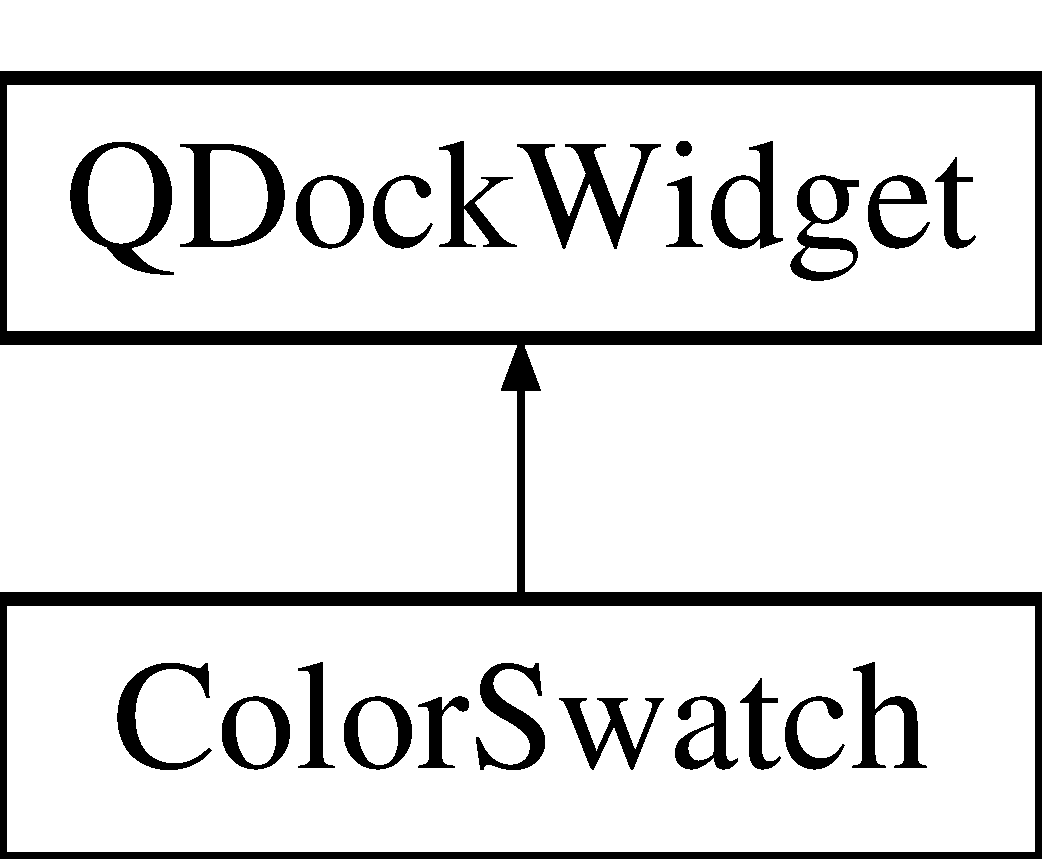
\includegraphics[height=2.000000cm]{class_color_swatch}
\end{center}
\end{figure}
\subsection*{Public Member Functions}
\begin{DoxyCompactItemize}
\item 
\hypertarget{class_color_swatch_a4e1aff7026fa62412bd35ea588cac508}{{\bfseries Color\-Swatch} (const Q\-String \&color\-Name, Q\-Widget $\ast$parent=0, Qt\-::\-Window\-Flags flags=0)}\label{class_color_swatch_a4e1aff7026fa62412bd35ea588cac508}

\item 
\hypertarget{class_color_swatch_ae967d9f7b8530ac4d07d5ed92e59599f}{void {\bfseries set\-Custom\-Size\-Hint} (const Q\-Size \&size)}\label{class_color_swatch_ae967d9f7b8530ac4d07d5ed92e59599f}

\end{DoxyCompactItemize}
\subsection*{Public Attributes}
\begin{DoxyCompactItemize}
\item 
\hypertarget{class_color_swatch_adeb8cbe648b985bb3231fb25927f8652}{Q\-Menu $\ast$ {\bfseries menu}}\label{class_color_swatch_adeb8cbe648b985bb3231fb25927f8652}

\item 
\hypertarget{class_color_swatch_a753ae92b7193a67376788434e58a3c52}{Q\-Action $\ast$ {\bfseries window\-Widget\-Action}}\label{class_color_swatch_a753ae92b7193a67376788434e58a3c52}

\end{DoxyCompactItemize}
\subsection*{Protected Member Functions}
\begin{DoxyCompactItemize}
\item 
\hypertarget{class_color_swatch_a0a5251704978879c5bc4456cd3240d78}{virtual void {\bfseries context\-Menu\-Event} (Q\-Context\-Menu\-Event $\ast$event)}\label{class_color_swatch_a0a5251704978879c5bc4456cd3240d78}

\item 
\hypertarget{class_color_swatch_a2cfb57e4968c2e8546ec0c8d9f5be0c2}{virtual void {\bfseries resize\-Event} (Q\-Resize\-Event $\ast$e)}\label{class_color_swatch_a2cfb57e4968c2e8546ec0c8d9f5be0c2}

\end{DoxyCompactItemize}


The documentation for this class was generated from the following files\-:\begin{DoxyCompactItemize}
\item 
colorswatch.\-h\item 
colorswatch.\-cpp\end{DoxyCompactItemize}

\hypertarget{class_erase_tool_base}{\section{Erase\-Tool\-Base Class Reference}
\label{class_erase_tool_base}\index{Erase\-Tool\-Base@{Erase\-Tool\-Base}}
}
Inheritance diagram for Erase\-Tool\-Base\-:\begin{figure}[H]
\begin{center}
\leavevmode
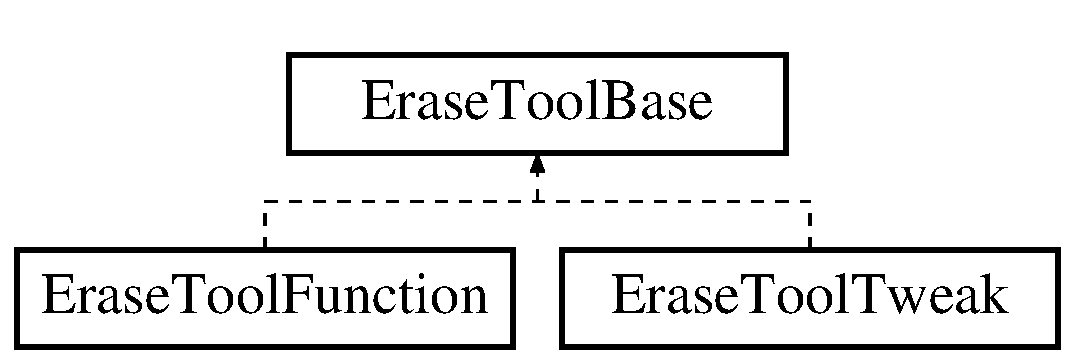
\includegraphics[height=2.000000cm]{class_erase_tool_base}
\end{center}
\end{figure}
\subsection*{Static Protected Attributes}
\begin{DoxyCompactItemize}
\item 
\hypertarget{class_erase_tool_base_a84600e8278accbb05e60f0c6f0a72364}{static int {\bfseries erase\-Size} =10}\label{class_erase_tool_base_a84600e8278accbb05e60f0c6f0a72364}

\item 
\hypertarget{class_erase_tool_base_a81e6975fa020c00e9e50cec440a96783}{static int {\bfseries erase\-Shape}}\label{class_erase_tool_base_a81e6975fa020c00e9e50cec440a96783}

\end{DoxyCompactItemize}


The documentation for this class was generated from the following files\-:\begin{DoxyCompactItemize}
\item 
toolbox.\-h\item 
toolbox.\-cpp\end{DoxyCompactItemize}

\hypertarget{class_erase_tool_function}{\section{Erase\-Tool\-Function Class Reference}
\label{class_erase_tool_function}\index{Erase\-Tool\-Function@{Erase\-Tool\-Function}}
}
Inheritance diagram for Erase\-Tool\-Function\-:\begin{figure}[H]
\begin{center}
\leavevmode
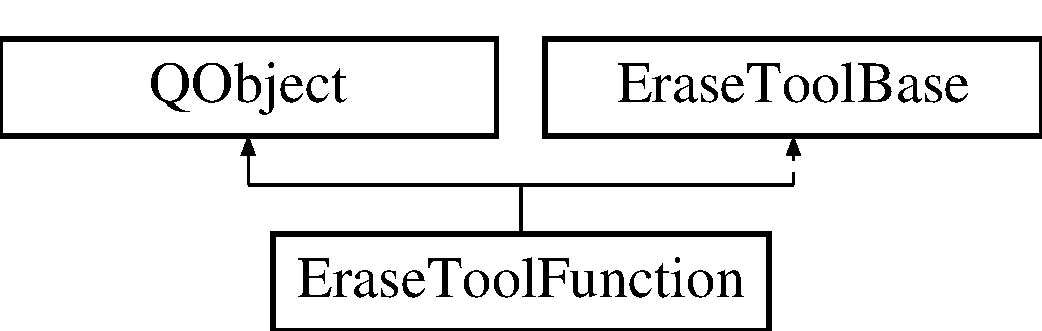
\includegraphics[height=2.000000cm]{class_erase_tool_function}
\end{center}
\end{figure}
\subsection*{Public Member Functions}
\begin{DoxyCompactItemize}
\item 
\hypertarget{class_erase_tool_function_ae8be235ad017c706c4ec7c01aa01fd0d}{{\bfseries Erase\-Tool\-Function} (Q\-Widget $\ast$parent)}\label{class_erase_tool_function_ae8be235ad017c706c4ec7c01aa01fd0d}

\item 
\hypertarget{class_erase_tool_function_acdee509cf5d65cdcf98aa0aa29ab22cc}{int {\bfseries get\-Erase\-Size} () const }\label{class_erase_tool_function_acdee509cf5d65cdcf98aa0aa29ab22cc}

\item 
\hypertarget{class_erase_tool_function_aebfa0e968e37a66f94c5843611193372}{bool {\bfseries get\-Erase\-Shape} () const }\label{class_erase_tool_function_aebfa0e968e37a66f94c5843611193372}

\end{DoxyCompactItemize}
\subsection*{Additional Inherited Members}


The documentation for this class was generated from the following files\-:\begin{DoxyCompactItemize}
\item 
toolbox.\-h\item 
toolbox.\-cpp\end{DoxyCompactItemize}

\hypertarget{class_erase_tool_tweak}{\section{Erase\-Tool\-Tweak Class Reference}
\label{class_erase_tool_tweak}\index{Erase\-Tool\-Tweak@{Erase\-Tool\-Tweak}}
}
Inheritance diagram for Erase\-Tool\-Tweak\-:\begin{figure}[H]
\begin{center}
\leavevmode
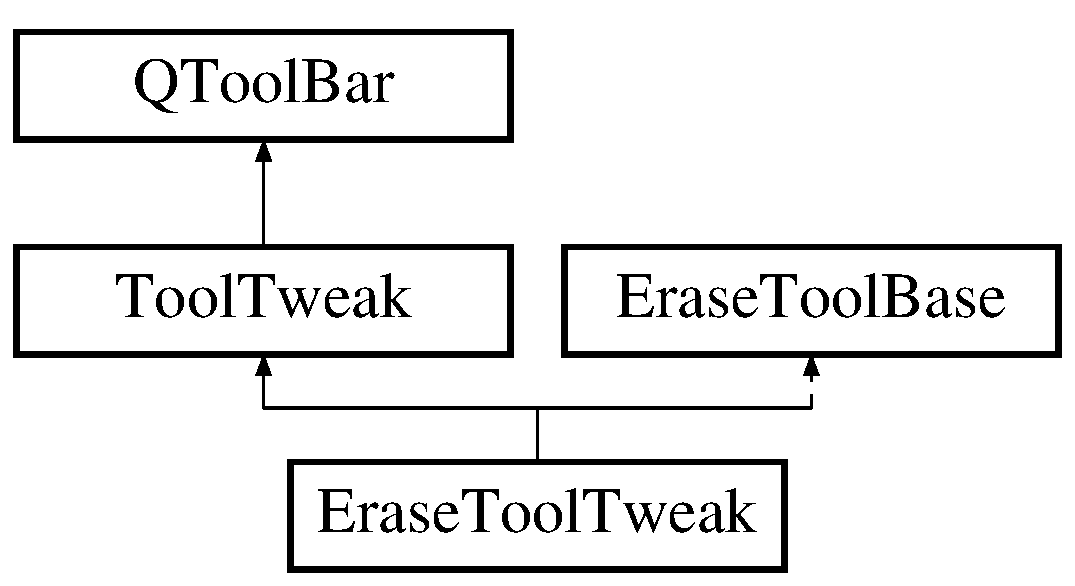
\includegraphics[height=3.000000cm]{class_erase_tool_tweak}
\end{center}
\end{figure}
\subsection*{Public Member Functions}
\begin{DoxyCompactItemize}
\item 
\hypertarget{class_erase_tool_tweak_a1c1c6c445c395c567c39ef36e2449646}{{\bfseries Erase\-Tool\-Tweak} (Q\-Widget $\ast$parent)}\label{class_erase_tool_tweak_a1c1c6c445c395c567c39ef36e2449646}

\end{DoxyCompactItemize}
\subsection*{Additional Inherited Members}


The documentation for this class was generated from the following files\-:\begin{DoxyCompactItemize}
\item 
toolbox.\-h\item 
toolbox.\-cpp\end{DoxyCompactItemize}

\hypertarget{class_lasso_tool_base}{\section{Lasso\-Tool\-Base Class Reference}
\label{class_lasso_tool_base}\index{Lasso\-Tool\-Base@{Lasso\-Tool\-Base}}
}
Inheritance diagram for Lasso\-Tool\-Base\-:\begin{figure}[H]
\begin{center}
\leavevmode
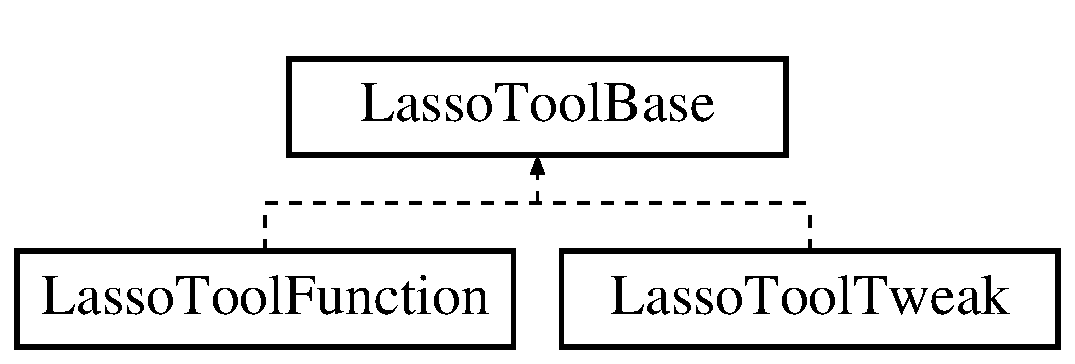
\includegraphics[height=2.000000cm]{class_lasso_tool_base}
\end{center}
\end{figure}
\subsection*{Static Protected Attributes}
\begin{DoxyCompactItemize}
\item 
\hypertarget{class_lasso_tool_base_aef6d6d2fd2e9994be1c6799e30e34f18}{static bool {\bfseries magnetic} =false}\label{class_lasso_tool_base_aef6d6d2fd2e9994be1c6799e30e34f18}

\end{DoxyCompactItemize}


The documentation for this class was generated from the following files\-:\begin{DoxyCompactItemize}
\item 
toolbox.\-h\item 
toolbox.\-cpp\end{DoxyCompactItemize}

\hypertarget{class_lasso_tool_function}{\section{Lasso\-Tool\-Function Class Reference}
\label{class_lasso_tool_function}\index{Lasso\-Tool\-Function@{Lasso\-Tool\-Function}}
}
Inheritance diagram for Lasso\-Tool\-Function\-:\begin{figure}[H]
\begin{center}
\leavevmode
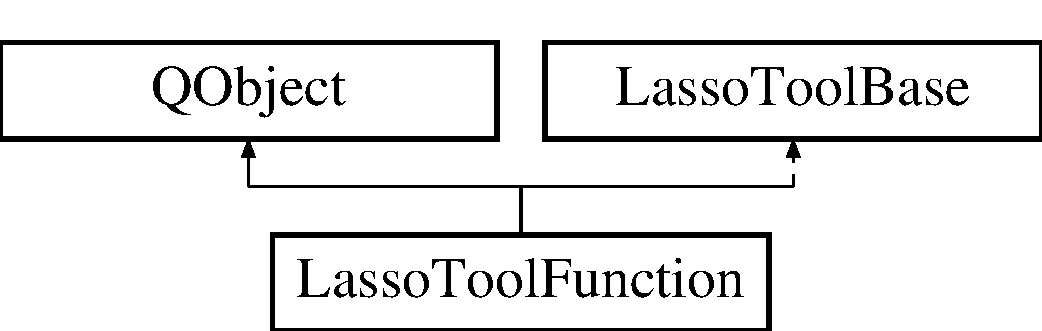
\includegraphics[height=2.000000cm]{class_lasso_tool_function}
\end{center}
\end{figure}
\subsection*{Public Member Functions}
\begin{DoxyCompactItemize}
\item 
\hypertarget{class_lasso_tool_function_ae6d52aec5bc8754d26c6eef37c1c6b08}{{\bfseries Lasso\-Tool\-Function} (Q\-Widget $\ast$parent)}\label{class_lasso_tool_function_ae6d52aec5bc8754d26c6eef37c1c6b08}

\item 
\hypertarget{class_lasso_tool_function_a5a463c428829f05f7e621e095073b36a}{bool {\bfseries get\-Magnetic} () const }\label{class_lasso_tool_function_a5a463c428829f05f7e621e095073b36a}

\end{DoxyCompactItemize}
\subsection*{Additional Inherited Members}


The documentation for this class was generated from the following files\-:\begin{DoxyCompactItemize}
\item 
toolbox.\-h\item 
toolbox.\-cpp\end{DoxyCompactItemize}

\hypertarget{class_lasso_tool_tweak}{\section{Lasso\-Tool\-Tweak Class Reference}
\label{class_lasso_tool_tweak}\index{Lasso\-Tool\-Tweak@{Lasso\-Tool\-Tweak}}
}
Inheritance diagram for Lasso\-Tool\-Tweak\-:\begin{figure}[H]
\begin{center}
\leavevmode
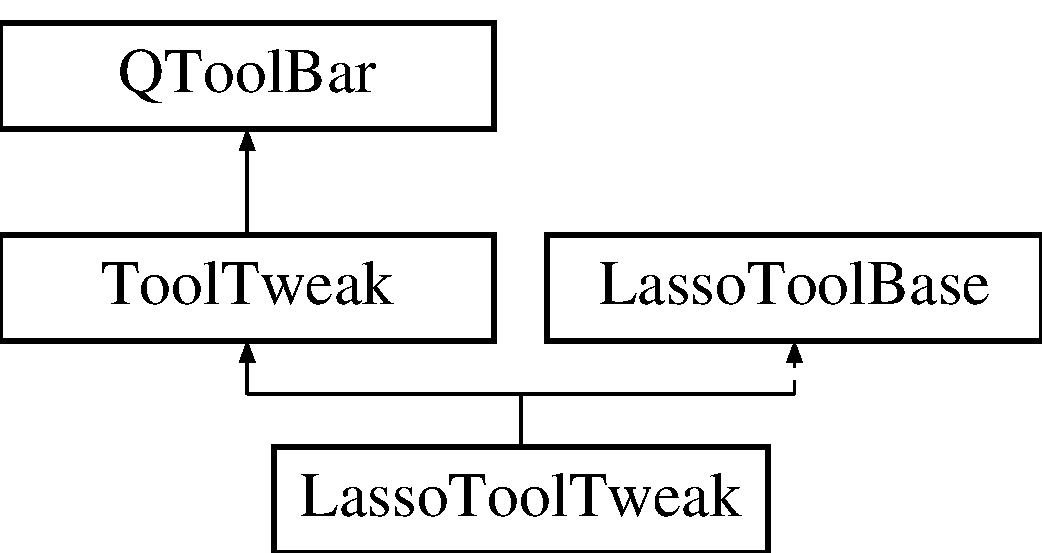
\includegraphics[height=3.000000cm]{class_lasso_tool_tweak}
\end{center}
\end{figure}
\subsection*{Public Member Functions}
\begin{DoxyCompactItemize}
\item 
\hypertarget{class_lasso_tool_tweak_a33e417e8efd7a9637853ae66cc25f5a7}{{\bfseries Lasso\-Tool\-Tweak} (Q\-Widget $\ast$parent)}\label{class_lasso_tool_tweak_a33e417e8efd7a9637853ae66cc25f5a7}

\end{DoxyCompactItemize}
\subsection*{Additional Inherited Members}


The documentation for this class was generated from the following files\-:\begin{DoxyCompactItemize}
\item 
toolbox.\-h\item 
toolbox.\-cpp\end{DoxyCompactItemize}

\hypertarget{struct_layer}{\section{Layer Struct Reference}
\label{struct_layer}\index{Layer@{Layer}}
}
\subsection*{Public Attributes}
\begin{DoxyCompactItemize}
\item 
\hypertarget{struct_layer_a69536f946617c35afb45929f8bc57062}{bool {\bfseries is\-Visible}}\label{struct_layer_a69536f946617c35afb45929f8bc57062}

\end{DoxyCompactItemize}


The documentation for this struct was generated from the following file\-:\begin{DoxyCompactItemize}
\item 
layerstack.\-h\end{DoxyCompactItemize}

\hypertarget{class_layer_stack}{\section{Layer\-Stack Class Reference}
\label{class_layer_stack}\index{Layer\-Stack@{Layer\-Stack}}
}
Inheritance diagram for Layer\-Stack\-:\begin{figure}[H]
\begin{center}
\leavevmode
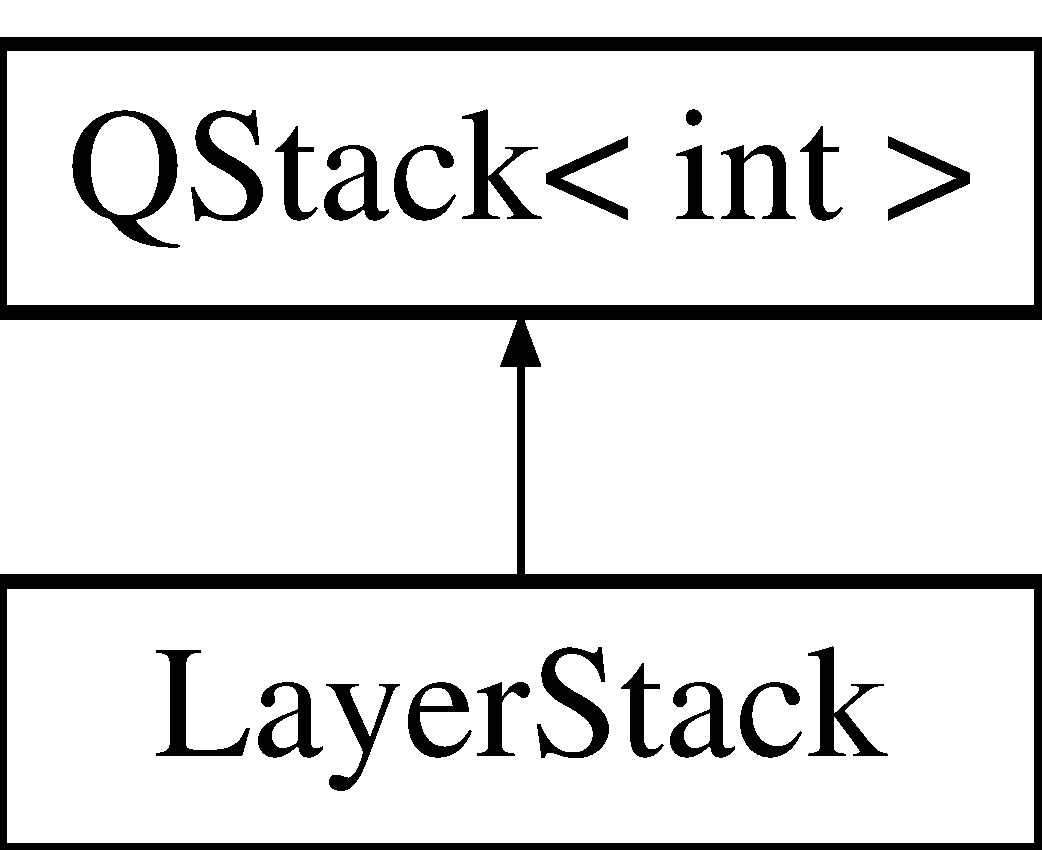
\includegraphics[height=2.000000cm]{class_layer_stack}
\end{center}
\end{figure}


The documentation for this class was generated from the following files\-:\begin{DoxyCompactItemize}
\item 
layerstack.\-h\item 
layerstack.\-cpp\end{DoxyCompactItemize}

\hypertarget{class_main_window}{\section{Main\-Window Class Reference}
\label{class_main_window}\index{Main\-Window@{Main\-Window}}
}


Create a \hyperlink{class_main_window}{Main\-Window}.  




{\ttfamily \#include $<$mainwindow.\-h$>$}

Inheritance diagram for Main\-Window\-:\begin{figure}[H]
\begin{center}
\leavevmode
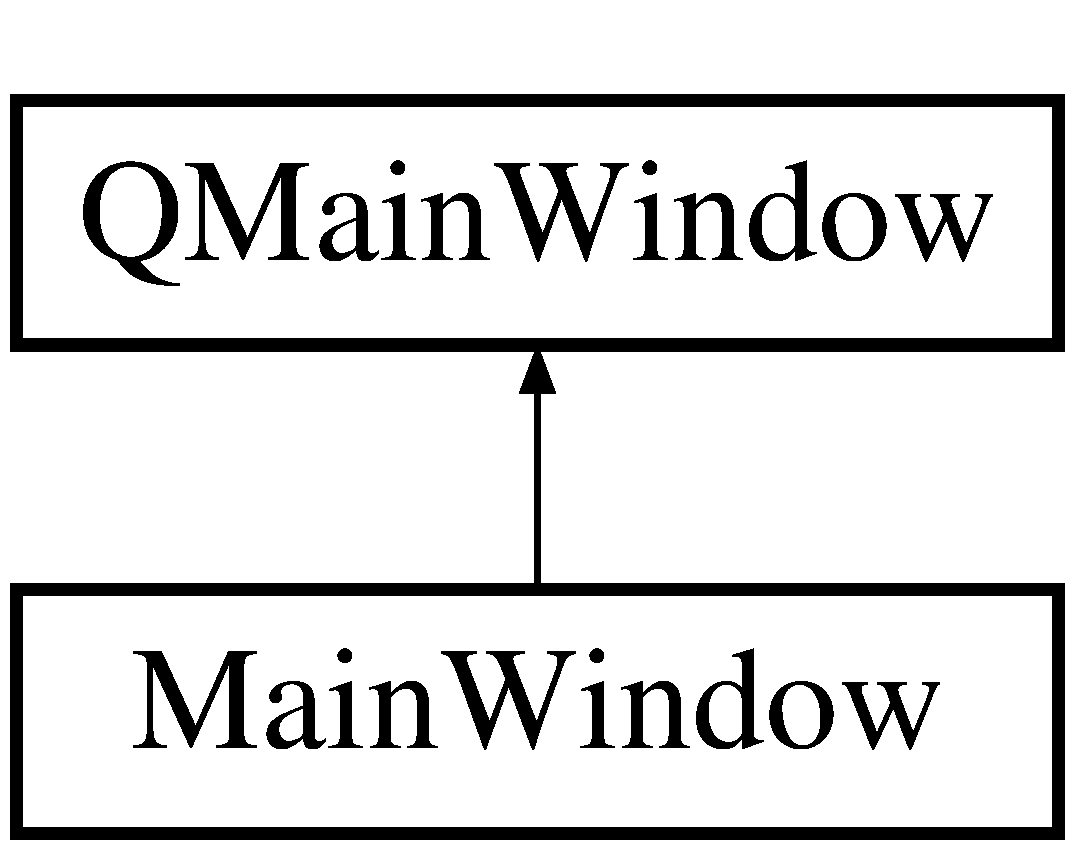
\includegraphics[height=2.000000cm]{class_main_window}
\end{center}
\end{figure}
\subsection*{Public Slots}
\begin{DoxyCompactItemize}
\item 
\hypertarget{class_main_window_a288b768c3c21a9171bdc56fe845ece8b}{void {\bfseries open\-File} ()}\label{class_main_window_a288b768c3c21a9171bdc56fe845ece8b}

\item 
\hypertarget{class_main_window_a464aaa4d378e7b2d814756a73d6e1ed6}{void {\bfseries save\-File} ()}\label{class_main_window_a464aaa4d378e7b2d814756a73d6e1ed6}

\item 
\hypertarget{class_main_window_addc822cb332163c0c182630f625732c8}{bool {\bfseries save\-Write} (const Q\-Byte\-Array)}\label{class_main_window_addc822cb332163c0c182630f625732c8}

\item 
\hypertarget{class_main_window_a44eb5d77b382a5acd4b0091f499f4352}{bool {\bfseries maybe\-Save} ()}\label{class_main_window_a44eb5d77b382a5acd4b0091f499f4352}

\item 
\hypertarget{class_main_window_aa00b272a4501c42347c0947579d7cf83}{void {\bfseries save\-Layout} ()}\label{class_main_window_aa00b272a4501c42347c0947579d7cf83}

\item 
\hypertarget{class_main_window_ae7b7947c2627ce667c69e8392f090f78}{void {\bfseries load\-Layout} ()}\label{class_main_window_ae7b7947c2627ce667c69e8392f090f78}

\item 
\hypertarget{class_main_window_a7be6a5d98970ac1a6296c6f9aee1e9bb}{void {\bfseries about} ()}\label{class_main_window_a7be6a5d98970ac1a6296c6f9aee1e9bb}

\end{DoxyCompactItemize}
\subsection*{Signals}
\begin{DoxyCompactItemize}
\item 
\hypertarget{class_main_window_abcf1574bf0f32094a3af3c8211b0b063}{void {\bfseries update\-Color\-Icon} (int, Q\-Color)}\label{class_main_window_abcf1574bf0f32094a3af3c8211b0b063}

\end{DoxyCompactItemize}
\subsection*{Public Member Functions}
\begin{DoxyCompactItemize}
\item 
\hyperlink{class_main_window_a8b244be8b7b7db1b08de2a2acb9409db}{Main\-Window} (Q\-Widget $\ast$parent=0)
\end{DoxyCompactItemize}
\subsection*{Protected Member Functions}
\begin{DoxyCompactItemize}
\item 
\hypertarget{class_main_window_a4e20a4a065fbb0e4d3532a45a0a91425}{void {\bfseries close\-Event} (Q\-Close\-Event $\ast$event)}\label{class_main_window_a4e20a4a065fbb0e4d3532a45a0a91425}

\end{DoxyCompactItemize}


\subsection{Detailed Description}
Create a \hyperlink{class_main_window}{Main\-Window}. 

\subsection{Constructor \& Destructor Documentation}
\hypertarget{class_main_window_a8b244be8b7b7db1b08de2a2acb9409db}{\index{Main\-Window@{Main\-Window}!Main\-Window@{Main\-Window}}
\index{Main\-Window@{Main\-Window}!MainWindow@{Main\-Window}}
\subsubsection[{Main\-Window}]{\setlength{\rightskip}{0pt plus 5cm}Main\-Window\-::\-Main\-Window (
\begin{DoxyParamCaption}
\item[{Q\-Widget $\ast$}]{parent = {\ttfamily 0}}
\end{DoxyParamCaption}
)}}\label{class_main_window_a8b244be8b7b7db1b08de2a2acb9409db}
Constructor 
\begin{DoxyParams}{Parameters}
{\em \mbox{[}\-Q\-Widget} & $\ast$parent\mbox{]} Parent Q\-Widget \\
\hline
\end{DoxyParams}


The documentation for this class was generated from the following files\-:\begin{DoxyCompactItemize}
\item 
mainwindow.\-h\item 
mainwindow.\-cpp\end{DoxyCompactItemize}

\hypertarget{class_marquee_tool_base}{\section{Marquee\-Tool\-Base Class Reference}
\label{class_marquee_tool_base}\index{Marquee\-Tool\-Base@{Marquee\-Tool\-Base}}
}
Inheritance diagram for Marquee\-Tool\-Base\-:\begin{figure}[H]
\begin{center}
\leavevmode
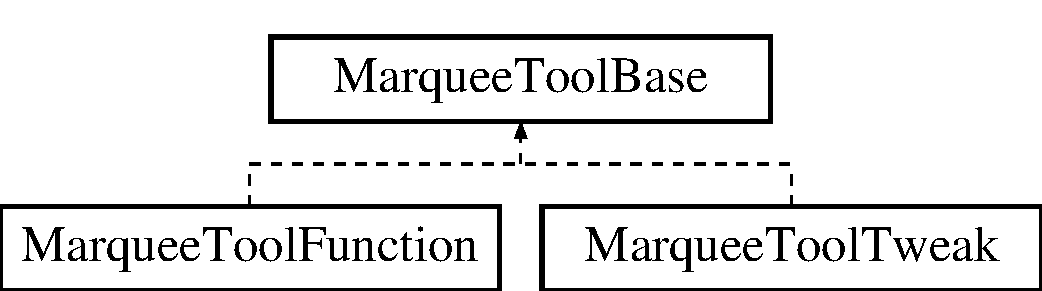
\includegraphics[height=2.000000cm]{class_marquee_tool_base}
\end{center}
\end{figure}
\subsection*{Static Protected Attributes}
\begin{DoxyCompactItemize}
\item 
\hypertarget{class_marquee_tool_base_aa174a70654de721265893e1dbe0863ca}{static int {\bfseries selection\-Type}}\label{class_marquee_tool_base_aa174a70654de721265893e1dbe0863ca}

\end{DoxyCompactItemize}


The documentation for this class was generated from the following files\-:\begin{DoxyCompactItemize}
\item 
toolbox.\-h\item 
toolbox.\-cpp\end{DoxyCompactItemize}

\hypertarget{class_marquee_tool_function}{\section{Marquee\-Tool\-Function Class Reference}
\label{class_marquee_tool_function}\index{Marquee\-Tool\-Function@{Marquee\-Tool\-Function}}
}
Inheritance diagram for Marquee\-Tool\-Function\-:\begin{figure}[H]
\begin{center}
\leavevmode
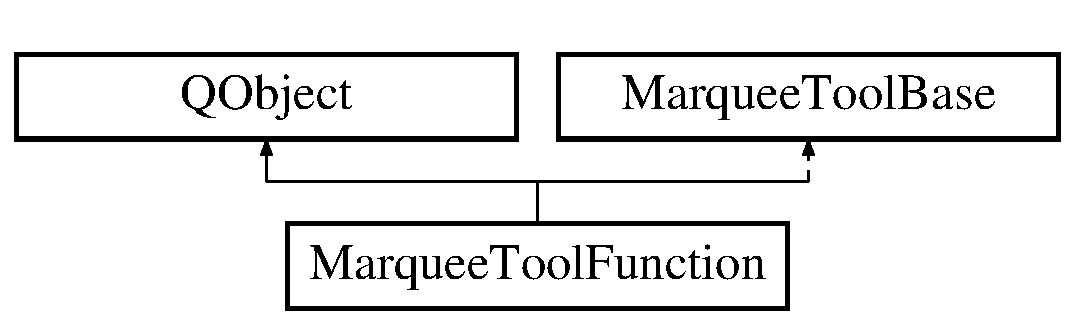
\includegraphics[height=2.000000cm]{class_marquee_tool_function}
\end{center}
\end{figure}
\subsection*{Public Member Functions}
\begin{DoxyCompactItemize}
\item 
\hypertarget{class_marquee_tool_function_a323f617feb6f5d0f3184855566856610}{{\bfseries Marquee\-Tool\-Function} (Q\-Widget $\ast$parent)}\label{class_marquee_tool_function_a323f617feb6f5d0f3184855566856610}

\item 
\hypertarget{class_marquee_tool_function_a56c0c5d191a8139627b4ccaf1d44bf9f}{int {\bfseries get\-Selection\-Type} () const }\label{class_marquee_tool_function_a56c0c5d191a8139627b4ccaf1d44bf9f}

\end{DoxyCompactItemize}
\subsection*{Additional Inherited Members}


The documentation for this class was generated from the following files\-:\begin{DoxyCompactItemize}
\item 
toolbox.\-h\item 
toolbox.\-cpp\end{DoxyCompactItemize}

\hypertarget{class_marquee_tool_tweak}{\section{Marquee\-Tool\-Tweak Class Reference}
\label{class_marquee_tool_tweak}\index{Marquee\-Tool\-Tweak@{Marquee\-Tool\-Tweak}}
}
Inheritance diagram for Marquee\-Tool\-Tweak\-:\begin{figure}[H]
\begin{center}
\leavevmode
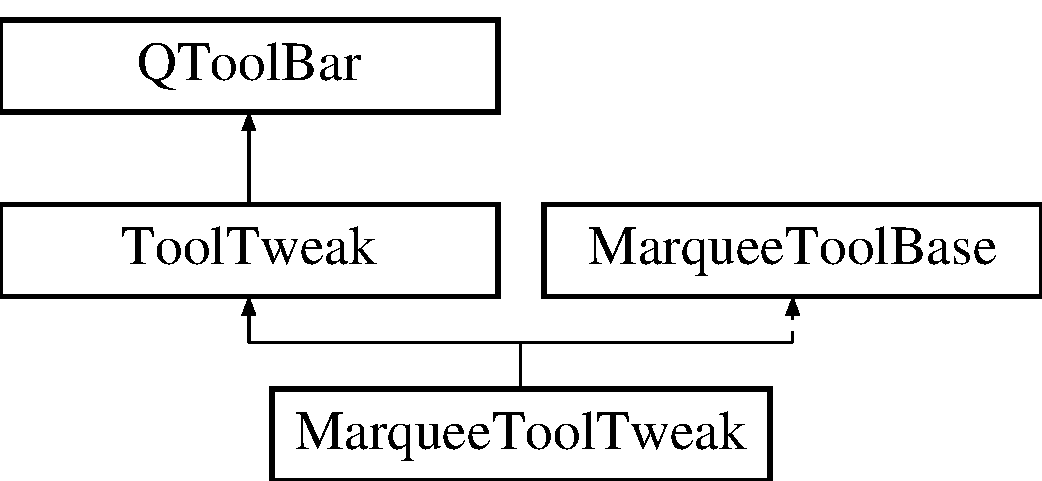
\includegraphics[height=3.000000cm]{class_marquee_tool_tweak}
\end{center}
\end{figure}
\subsection*{Public Member Functions}
\begin{DoxyCompactItemize}
\item 
\hypertarget{class_marquee_tool_tweak_ac05c2e399fc62162142b43d3bcef605a}{{\bfseries Marquee\-Tool\-Tweak} (Q\-Widget $\ast$parent)}\label{class_marquee_tool_tweak_ac05c2e399fc62162142b43d3bcef605a}

\end{DoxyCompactItemize}
\subsection*{Additional Inherited Members}


The documentation for this class was generated from the following files\-:\begin{DoxyCompactItemize}
\item 
toolbox.\-h\item 
toolbox.\-cpp\end{DoxyCompactItemize}

\hypertarget{class_pen_tool_base}{\section{Pen\-Tool\-Base Class Reference}
\label{class_pen_tool_base}\index{Pen\-Tool\-Base@{Pen\-Tool\-Base}}
}
Inheritance diagram for Pen\-Tool\-Base\-:\begin{figure}[H]
\begin{center}
\leavevmode
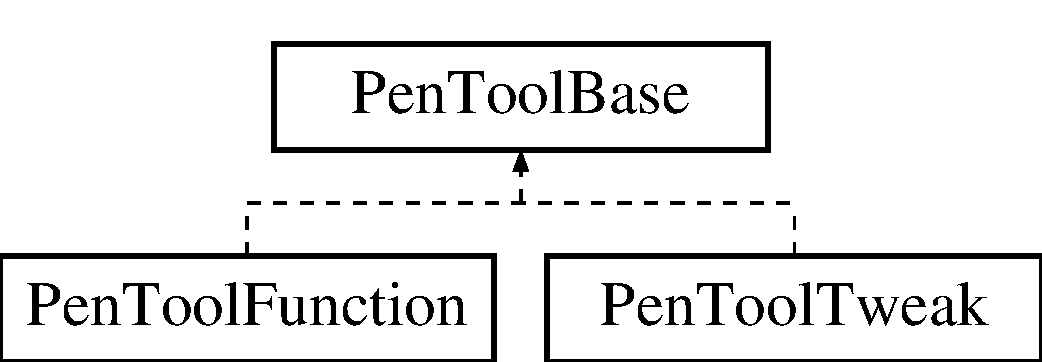
\includegraphics[height=2.000000cm]{class_pen_tool_base}
\end{center}
\end{figure}


The documentation for this class was generated from the following file\-:\begin{DoxyCompactItemize}
\item 
toolbox.\-h\end{DoxyCompactItemize}

\hypertarget{class_pen_tool_function}{\section{Pen\-Tool\-Function Class Reference}
\label{class_pen_tool_function}\index{Pen\-Tool\-Function@{Pen\-Tool\-Function}}
}
Inheritance diagram for Pen\-Tool\-Function\-:\begin{figure}[H]
\begin{center}
\leavevmode
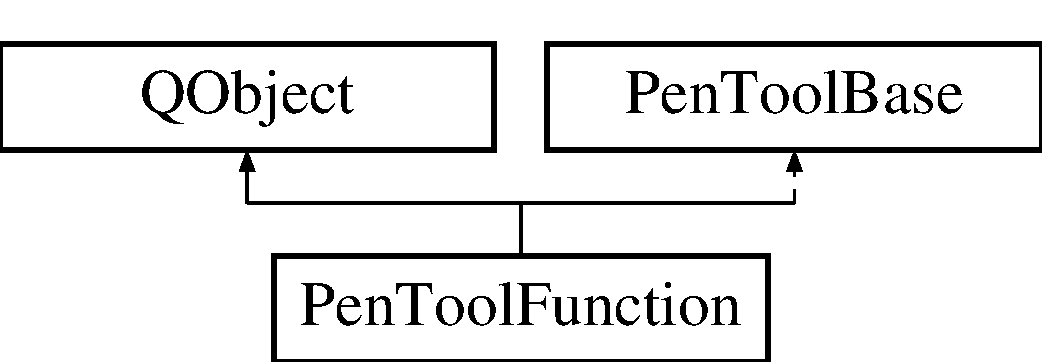
\includegraphics[height=2.000000cm]{class_pen_tool_function}
\end{center}
\end{figure}
\subsection*{Public Slots}
\begin{DoxyCompactItemize}
\item 
\hypertarget{class_pen_tool_function_ad429ee478c88fbe6fcde019697cef33a}{void {\bfseries clear\-Points} ()}\label{class_pen_tool_function_ad429ee478c88fbe6fcde019697cef33a}

\end{DoxyCompactItemize}
\subsection*{Signals}
\begin{DoxyCompactItemize}
\item 
\hypertarget{class_pen_tool_function_a2ac783638b62266d6a28710df44b9df6}{void {\bfseries make\-Selection} ()}\label{class_pen_tool_function_a2ac783638b62266d6a28710df44b9df6}

\item 
\hypertarget{class_pen_tool_function_aa7f05839c3047455cec70c77d7ca4b64}{void {\bfseries stroke\-Path} ()}\label{class_pen_tool_function_aa7f05839c3047455cec70c77d7ca4b64}

\item 
\hypertarget{class_pen_tool_function_ad7850683e22b794480618b0783dd8860}{void {\bfseries fill\-Path} ()}\label{class_pen_tool_function_ad7850683e22b794480618b0783dd8860}

\end{DoxyCompactItemize}
\subsection*{Public Member Functions}
\begin{DoxyCompactItemize}
\item 
\hypertarget{class_pen_tool_function_a579c797d3acdd3e89b956324c10eee19}{{\bfseries Pen\-Tool\-Function} (Q\-Widget $\ast$parent)}\label{class_pen_tool_function_a579c797d3acdd3e89b956324c10eee19}

\end{DoxyCompactItemize}
\subsection*{Public Attributes}
\begin{DoxyCompactItemize}
\item 
\hypertarget{class_pen_tool_function_aa19ea9aad1259a20773d684e89dbbe1b}{Hover\-Points $\ast$ {\bfseries pen\-Handler}}\label{class_pen_tool_function_aa19ea9aad1259a20773d684e89dbbe1b}

\item 
\hypertarget{class_pen_tool_function_a8b1e4989a925ecb9539dea62bf1d1d16}{Q\-Polygon\-F {\bfseries pen\-Handler\-Control}}\label{class_pen_tool_function_a8b1e4989a925ecb9539dea62bf1d1d16}

\item 
\hypertarget{class_pen_tool_function_a1e3c29909108f341004171395ca13bc8}{Q\-Menu $\ast$ {\bfseries pen\-Menu}}\label{class_pen_tool_function_a1e3c29909108f341004171395ca13bc8}

\end{DoxyCompactItemize}


The documentation for this class was generated from the following files\-:\begin{DoxyCompactItemize}
\item 
toolbox.\-h\item 
toolbox.\-cpp\end{DoxyCompactItemize}

\hypertarget{class_pen_tool_tweak}{\section{Pen\-Tool\-Tweak Class Reference}
\label{class_pen_tool_tweak}\index{Pen\-Tool\-Tweak@{Pen\-Tool\-Tweak}}
}
Inheritance diagram for Pen\-Tool\-Tweak\-:\begin{figure}[H]
\begin{center}
\leavevmode
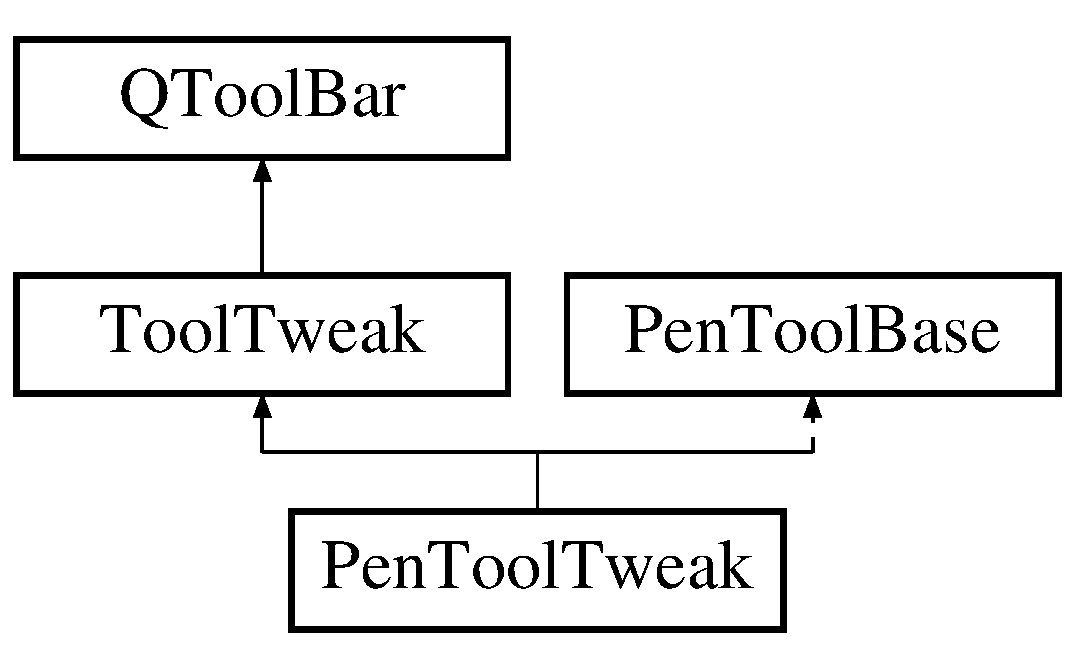
\includegraphics[height=3.000000cm]{class_pen_tool_tweak}
\end{center}
\end{figure}
\subsection*{Public Member Functions}
\begin{DoxyCompactItemize}
\item 
\hypertarget{class_pen_tool_tweak_abed45b54424ce19cb7b8dd73de9233e5}{{\bfseries Pen\-Tool\-Tweak} (Q\-Widget $\ast$parent)}\label{class_pen_tool_tweak_abed45b54424ce19cb7b8dd73de9233e5}

\end{DoxyCompactItemize}


The documentation for this class was generated from the following files\-:\begin{DoxyCompactItemize}
\item 
toolbox.\-h\item 
toolbox.\-cpp\end{DoxyCompactItemize}

\hypertarget{class_scribble_area}{\section{Scribble\-Area Class Reference}
\label{class_scribble_area}\index{Scribble\-Area@{Scribble\-Area}}
}


\mbox{[}0\mbox{]}  




{\ttfamily \#include $<$scribblearea.\-h$>$}

Inheritance diagram for Scribble\-Area\-:\begin{figure}[H]
\begin{center}
\leavevmode
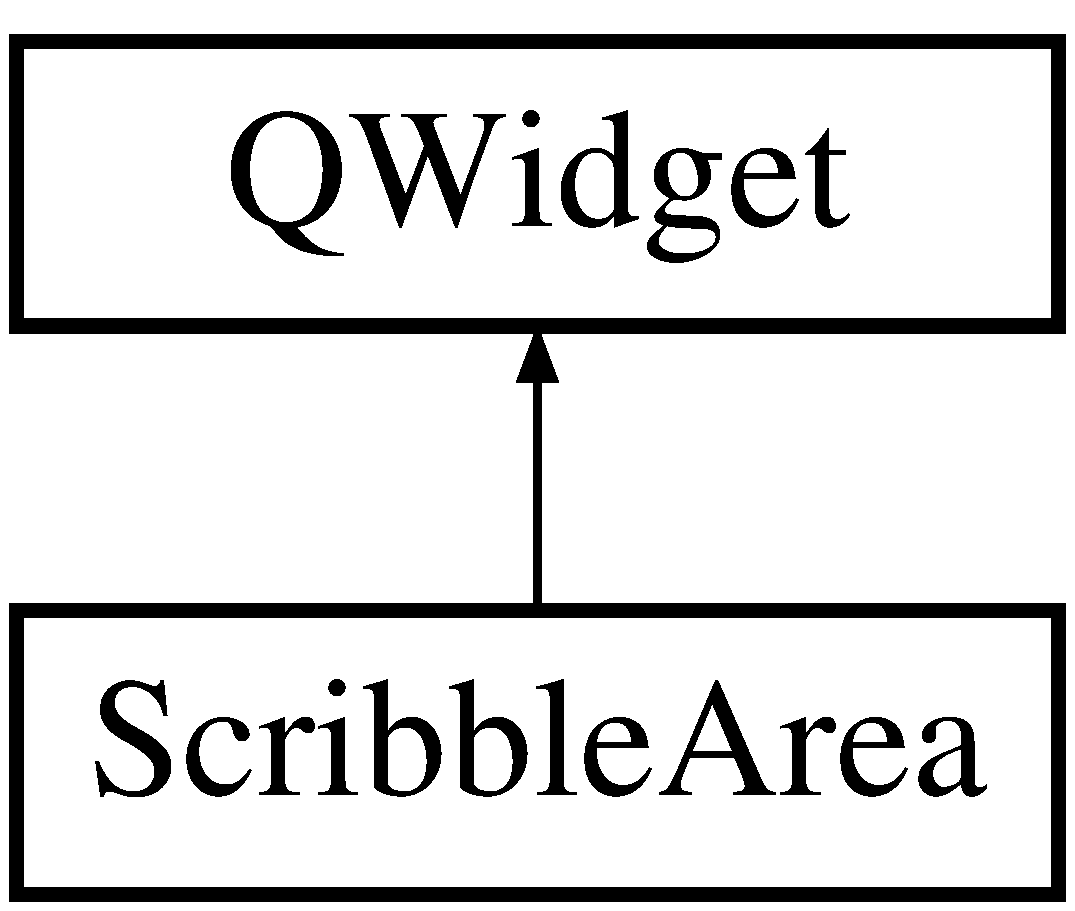
\includegraphics[height=2.000000cm]{class_scribble_area}
\end{center}
\end{figure}
\subsection*{Public Slots}
\begin{DoxyCompactItemize}
\item 
\hypertarget{class_scribble_area_a331b4c8f2b811671e140f75dc31a2c39}{void {\bfseries update\-Display} (int changed\-Image\-Num)}\label{class_scribble_area_a331b4c8f2b811671e140f75dc31a2c39}

\item 
\hypertarget{class_scribble_area_a07899960089b06f36d40ddcbf087d18f}{void {\bfseries update\-Cursor} ()}\label{class_scribble_area_a07899960089b06f36d40ddcbf087d18f}

\item 
\hypertarget{class_scribble_area_a1df2c552892d9d8c3e5e5f04f33f5610}{void {\bfseries make\-Selection} (void)}\label{class_scribble_area_a1df2c552892d9d8c3e5e5f04f33f5610}

\item 
\hypertarget{class_scribble_area_ab368bb43f8377a0bc022517b7238f677}{void {\bfseries stroke\-Selected\-Area} (void)}\label{class_scribble_area_ab368bb43f8377a0bc022517b7238f677}

\item 
\hypertarget{class_scribble_area_aaf30782668dfa40aea56062a31f84826}{void {\bfseries fill\-Selected\-Area} (void)}\label{class_scribble_area_aaf30782668dfa40aea56062a31f84826}

\item 
\hypertarget{class_scribble_area_a0c33d7376960578c2cc39d9bfb153ad2}{void {\bfseries black\-And\-White} (void)}\label{class_scribble_area_a0c33d7376960578c2cc39d9bfb153ad2}

\item 
void \hyperlink{class_scribble_area_a5b5545e0f7fbc6b6ee901fac13830a6e}{gaussian\-Blur} (void)
\item 
void \hyperlink{class_scribble_area_aff9034e3ddaae1296a3aab8fdb30fd30}{canny\-Edge} (void)
\item 
void \hyperlink{class_scribble_area_ad413c39ee40eb142f80dcb283d29c86a}{erode\-Filter} (void)
\item 
void \hyperlink{class_scribble_area_a77ea883ff6313a019d53b42a1254adad}{dilate\-Filter} (void)
\item 
\hypertarget{class_scribble_area_ab132e409c1e8932133c914413d498453}{void {\bfseries grabcut\-Filter} (void)}\label{class_scribble_area_ab132e409c1e8932133c914413d498453}

\end{DoxyCompactItemize}
\subsection*{Public Member Functions}
\begin{DoxyCompactItemize}
\item 
\hyperlink{class_scribble_area_a3560f2a44b46531591a1f4b1e42ea86f}{Scribble\-Area} (Q\-Widget $\ast$parent=0)
\item 
\hypertarget{class_scribble_area_a39eccfe97fab1b788cc873d5de7fce46}{bool {\bfseries is\-Modified} () const }\label{class_scribble_area_a39eccfe97fab1b788cc873d5de7fce46}

\item 
\hypertarget{class_scribble_area_a654dbfae57876cc88bcc08f6fc06611e}{void {\bfseries set\-Modified} (bool value)}\label{class_scribble_area_a654dbfae57876cc88bcc08f6fc06611e}

\item 
\hypertarget{class_scribble_area_acb1671a94370515af09a2530170d594f}{void {\bfseries set\-Tool\-Type} (Tool\-Type\-::tool\-Type type)}\label{class_scribble_area_acb1671a94370515af09a2530170d594f}

\item 
\hypertarget{class_scribble_area_a6a7a010f7d73e8ceaed52e1253dbcdd0}{void {\bfseries set\-Fg\-Color} (Q\-Color color)}\label{class_scribble_area_a6a7a010f7d73e8ceaed52e1253dbcdd0}

\item 
\hypertarget{class_scribble_area_a9f858c56ae7f5e06a11dbc022c8caf02}{void {\bfseries set\-Bg\-Color} (Q\-Color color)}\label{class_scribble_area_a9f858c56ae7f5e06a11dbc022c8caf02}

\item 
\hypertarget{class_scribble_area_af463a9e82b63ca30be22df4c01e8436a}{void {\bfseries select\-All} (void)}\label{class_scribble_area_af463a9e82b63ca30be22df4c01e8436a}

\item 
\hypertarget{class_scribble_area_a0c9f70e3ce6d57c25dd641cb7e14bb38}{void {\bfseries Apply\-Tool\-Function} (Q\-Point last\-Point, Q\-Point current\-Point)}\label{class_scribble_area_a0c9f70e3ce6d57c25dd641cb7e14bb38}

\item 
\hypertarget{class_scribble_area_ae4e8671f48893ab00eefbf2b6e843621}{void {\bfseries Apply\-Tool\-Function} (Q\-Point current\-Point)}\label{class_scribble_area_ae4e8671f48893ab00eefbf2b6e843621}

\item 
\hypertarget{class_scribble_area_a42255c7a44479e447a43bf26e7a89822}{void {\bfseries Apply\-Tool\-Function} ()}\label{class_scribble_area_a42255c7a44479e447a43bf26e7a89822}

\item 
bool \hyperlink{class_scribble_area_afdce32fa1f5d3220987d4983e8a43e1e}{open\-Image} (const Q\-String \&file\-Name)
\begin{DoxyCompactList}\small\item\em \mbox{[}1\mbox{]} \end{DoxyCompactList}\item 
bool \hyperlink{class_scribble_area_a9496b9970942db6abfea836e6bf56ee4}{save\-Image} (const Q\-String \&file\-Name, const char $\ast$file\-Format)
\begin{DoxyCompactList}\small\item\em \mbox{[}2\mbox{]} \end{DoxyCompactList}\item 
void \hyperlink{class_scribble_area_a60cb2e490f094334b8ccb48b636bb67e}{draw\-Line\-To} (Q\-Point last\-Point, Q\-Point current\-Point)
\item 
\hypertarget{class_scribble_area_af968a1bb4a81acf6a2462fd3ecb7c725}{void {\bfseries resize\-Image} (Q\-Image $\ast$image, const Q\-Size \&new\-Size)}\label{class_scribble_area_af968a1bb4a81acf6a2462fd3ecb7c725}

\item 
\hypertarget{class_scribble_area_aefa0ba0130c92343894b2dfefd8374cd}{void {\bfseries delete\-Selected\-Area} (void)}\label{class_scribble_area_aefa0ba0130c92343894b2dfefd8374cd}

\item 
\hypertarget{class_scribble_area_a23a1bc070ce18355bdc91464ec5fd8fe}{void {\bfseries set\-Transform\-Selection\-State} (void)}\label{class_scribble_area_a23a1bc070ce18355bdc91464ec5fd8fe}

\end{DoxyCompactItemize}
\subsection*{Protected Member Functions}
\begin{DoxyCompactItemize}
\item 
\hypertarget{class_scribble_area_a7646e72c61ec6a1eeda468fb6dfa66f1}{void {\bfseries mouse\-Press\-Event} (Q\-Mouse\-Event $\ast$event)}\label{class_scribble_area_a7646e72c61ec6a1eeda468fb6dfa66f1}

\item 
\hypertarget{class_scribble_area_ae98981b6c07de07afdc39d57810e945b}{void {\bfseries mouse\-Move\-Event} (Q\-Mouse\-Event $\ast$event)}\label{class_scribble_area_ae98981b6c07de07afdc39d57810e945b}

\item 
\hypertarget{class_scribble_area_a991eb6ab4ac21895973bc9d81b84a30e}{void {\bfseries mouse\-Release\-Event} (Q\-Mouse\-Event $\ast$event)}\label{class_scribble_area_a991eb6ab4ac21895973bc9d81b84a30e}

\item 
\hypertarget{class_scribble_area_abf143b77fc6dac887cd71ce7488fa804}{void {\bfseries enter\-Event} (Q\-Event $\ast$event)}\label{class_scribble_area_abf143b77fc6dac887cd71ce7488fa804}

\item 
void \hyperlink{class_scribble_area_a126a30e3659f6c1cdc202f10fce7e5d9}{paint\-Event} (Q\-Paint\-Event $\ast$event)
\begin{DoxyCompactList}\small\item\em \mbox{[}12\mbox{]} //! \mbox{[}13\mbox{]} \end{DoxyCompactList}\item 
void \hyperlink{class_scribble_area_aaf6be24625a5f0fe1e4a3b8eecb07575}{resize\-Event} (Q\-Resize\-Event $\ast$event)
\begin{DoxyCompactList}\small\item\em \mbox{[}14\mbox{]} \end{DoxyCompactList}\item 
\hypertarget{class_scribble_area_a3ed554609fd0eb635760ab75abe81479}{void {\bfseries key\-Press\-Event} (Q\-Key\-Event $\ast$event)}\label{class_scribble_area_a3ed554609fd0eb635760ab75abe81479}

\item 
\hypertarget{class_scribble_area_ace1abdc60eb03298dbcc1de3833bd80a}{void {\bfseries context\-Menu\-Event} (Q\-Context\-Menu\-Event $\ast$event)}\label{class_scribble_area_ace1abdc60eb03298dbcc1de3833bd80a}

\end{DoxyCompactItemize}


\subsection{Detailed Description}
\mbox{[}0\mbox{]} 

\subsection{Constructor \& Destructor Documentation}
\hypertarget{class_scribble_area_a3560f2a44b46531591a1f4b1e42ea86f}{\index{Scribble\-Area@{Scribble\-Area}!Scribble\-Area@{Scribble\-Area}}
\index{Scribble\-Area@{Scribble\-Area}!ScribbleArea@{Scribble\-Area}}
\subsubsection[{Scribble\-Area}]{\setlength{\rightskip}{0pt plus 5cm}Scribble\-Area\-::\-Scribble\-Area (
\begin{DoxyParamCaption}
\item[{Q\-Widget $\ast$}]{parent = {\ttfamily 0}}
\end{DoxyParamCaption}
)}}\label{class_scribble_area_a3560f2a44b46531591a1f4b1e42ea86f}
\mbox{[}0\mbox{]} 

\subsection{Member Function Documentation}
\hypertarget{class_scribble_area_aff9034e3ddaae1296a3aab8fdb30fd30}{\index{Scribble\-Area@{Scribble\-Area}!canny\-Edge@{canny\-Edge}}
\index{canny\-Edge@{canny\-Edge}!ScribbleArea@{Scribble\-Area}}
\subsubsection[{canny\-Edge}]{\setlength{\rightskip}{0pt plus 5cm}void Scribble\-Area\-::canny\-Edge (
\begin{DoxyParamCaption}
\item[{void}]{}
\end{DoxyParamCaption}
)\hspace{0.3cm}{\ttfamily [slot]}}}\label{class_scribble_area_aff9034e3ddaae1296a3aab8fdb30fd30}
\begin{DoxyNote}{Note}
Range need to be set 
\end{DoxyNote}
\hypertarget{class_scribble_area_a77ea883ff6313a019d53b42a1254adad}{\index{Scribble\-Area@{Scribble\-Area}!dilate\-Filter@{dilate\-Filter}}
\index{dilate\-Filter@{dilate\-Filter}!ScribbleArea@{Scribble\-Area}}
\subsubsection[{dilate\-Filter}]{\setlength{\rightskip}{0pt plus 5cm}void Scribble\-Area\-::dilate\-Filter (
\begin{DoxyParamCaption}
\item[{void}]{}
\end{DoxyParamCaption}
)\hspace{0.3cm}{\ttfamily [slot]}}}\label{class_scribble_area_a77ea883ff6313a019d53b42a1254adad}
\begin{DoxyNote}{Note}
Range need to be set 
\end{DoxyNote}
\hypertarget{class_scribble_area_a60cb2e490f094334b8ccb48b636bb67e}{\index{Scribble\-Area@{Scribble\-Area}!draw\-Line\-To@{draw\-Line\-To}}
\index{draw\-Line\-To@{draw\-Line\-To}!ScribbleArea@{Scribble\-Area}}
\subsubsection[{draw\-Line\-To}]{\setlength{\rightskip}{0pt plus 5cm}void Scribble\-Area\-::draw\-Line\-To (
\begin{DoxyParamCaption}
\item[{Q\-Point}]{last\-Point, }
\item[{Q\-Point}]{current\-Point}
\end{DoxyParamCaption}
)}}\label{class_scribble_area_a60cb2e490f094334b8ccb48b636bb67e}
cv\-Scalar(b, g, r, a); \hypertarget{class_scribble_area_ad413c39ee40eb142f80dcb283d29c86a}{\index{Scribble\-Area@{Scribble\-Area}!erode\-Filter@{erode\-Filter}}
\index{erode\-Filter@{erode\-Filter}!ScribbleArea@{Scribble\-Area}}
\subsubsection[{erode\-Filter}]{\setlength{\rightskip}{0pt plus 5cm}void Scribble\-Area\-::erode\-Filter (
\begin{DoxyParamCaption}
\item[{void}]{}
\end{DoxyParamCaption}
)\hspace{0.3cm}{\ttfamily [slot]}}}\label{class_scribble_area_ad413c39ee40eb142f80dcb283d29c86a}
\begin{DoxyNote}{Note}
Range need to be set 
\end{DoxyNote}
\hypertarget{class_scribble_area_a5b5545e0f7fbc6b6ee901fac13830a6e}{\index{Scribble\-Area@{Scribble\-Area}!gaussian\-Blur@{gaussian\-Blur}}
\index{gaussian\-Blur@{gaussian\-Blur}!ScribbleArea@{Scribble\-Area}}
\subsubsection[{gaussian\-Blur}]{\setlength{\rightskip}{0pt plus 5cm}void Scribble\-Area\-::gaussian\-Blur (
\begin{DoxyParamCaption}
\item[{void}]{}
\end{DoxyParamCaption}
)\hspace{0.3cm}{\ttfamily [slot]}}}\label{class_scribble_area_a5b5545e0f7fbc6b6ee901fac13830a6e}
\begin{DoxyNote}{Note}
Value step need to be set

Range need to be set 
\end{DoxyNote}
\hypertarget{class_scribble_area_afdce32fa1f5d3220987d4983e8a43e1e}{\index{Scribble\-Area@{Scribble\-Area}!open\-Image@{open\-Image}}
\index{open\-Image@{open\-Image}!ScribbleArea@{Scribble\-Area}}
\subsubsection[{open\-Image}]{\setlength{\rightskip}{0pt plus 5cm}bool Scribble\-Area\-::open\-Image (
\begin{DoxyParamCaption}
\item[{const Q\-String \&}]{file\-Name}
\end{DoxyParamCaption}
)}}\label{class_scribble_area_afdce32fa1f5d3220987d4983e8a43e1e}


\mbox{[}1\mbox{]} 

\mbox{[}1\mbox{]} //! \mbox{[}2\mbox{]} \hypertarget{class_scribble_area_a126a30e3659f6c1cdc202f10fce7e5d9}{\index{Scribble\-Area@{Scribble\-Area}!paint\-Event@{paint\-Event}}
\index{paint\-Event@{paint\-Event}!ScribbleArea@{Scribble\-Area}}
\subsubsection[{paint\-Event}]{\setlength{\rightskip}{0pt plus 5cm}void Scribble\-Area\-::paint\-Event (
\begin{DoxyParamCaption}
\item[{Q\-Paint\-Event $\ast$}]{event}
\end{DoxyParamCaption}
)\hspace{0.3cm}{\ttfamily [protected]}}}\label{class_scribble_area_a126a30e3659f6c1cdc202f10fce7e5d9}


\mbox{[}12\mbox{]} //! \mbox{[}13\mbox{]} 

\mbox{[}13\mbox{]} //! \mbox{[}14\mbox{]} \begin{DoxyNote}{Note}
can be optimized, update one small area one time 
\end{DoxyNote}
\hypertarget{class_scribble_area_aaf6be24625a5f0fe1e4a3b8eecb07575}{\index{Scribble\-Area@{Scribble\-Area}!resize\-Event@{resize\-Event}}
\index{resize\-Event@{resize\-Event}!ScribbleArea@{Scribble\-Area}}
\subsubsection[{resize\-Event}]{\setlength{\rightskip}{0pt plus 5cm}void Scribble\-Area\-::resize\-Event (
\begin{DoxyParamCaption}
\item[{Q\-Resize\-Event $\ast$}]{event}
\end{DoxyParamCaption}
)\hspace{0.3cm}{\ttfamily [protected]}}}\label{class_scribble_area_aaf6be24625a5f0fe1e4a3b8eecb07575}


\mbox{[}14\mbox{]} 

\mbox{[}15\mbox{]} \mbox{[}15\mbox{]} //! \mbox{[}16\mbox{]} \hypertarget{class_scribble_area_a9496b9970942db6abfea836e6bf56ee4}{\index{Scribble\-Area@{Scribble\-Area}!save\-Image@{save\-Image}}
\index{save\-Image@{save\-Image}!ScribbleArea@{Scribble\-Area}}
\subsubsection[{save\-Image}]{\setlength{\rightskip}{0pt plus 5cm}bool Scribble\-Area\-::save\-Image (
\begin{DoxyParamCaption}
\item[{const Q\-String \&}]{file\-Name, }
\item[{const char $\ast$}]{file\-Format}
\end{DoxyParamCaption}
)}}\label{class_scribble_area_a9496b9970942db6abfea836e6bf56ee4}


\mbox{[}2\mbox{]} 

\mbox{[}3\mbox{]} \mbox{[}3\mbox{]} //! \mbox{[}4\mbox{]} \mbox{[}4\mbox{]} \begin{DoxyNote}{Note}
Save image is not implemented 
\end{DoxyNote}


The documentation for this class was generated from the following files\-:\begin{DoxyCompactItemize}
\item 
scribblearea.\-h\item 
opencvprocess.\-cpp\item 
scribblearea.\-cpp\end{DoxyCompactItemize}

\hypertarget{class_tool_bar}{\section{Tool\-Bar Class Reference}
\label{class_tool_bar}\index{Tool\-Bar@{Tool\-Bar}}
}
Inheritance diagram for Tool\-Bar\-:\begin{figure}[H]
\begin{center}
\leavevmode
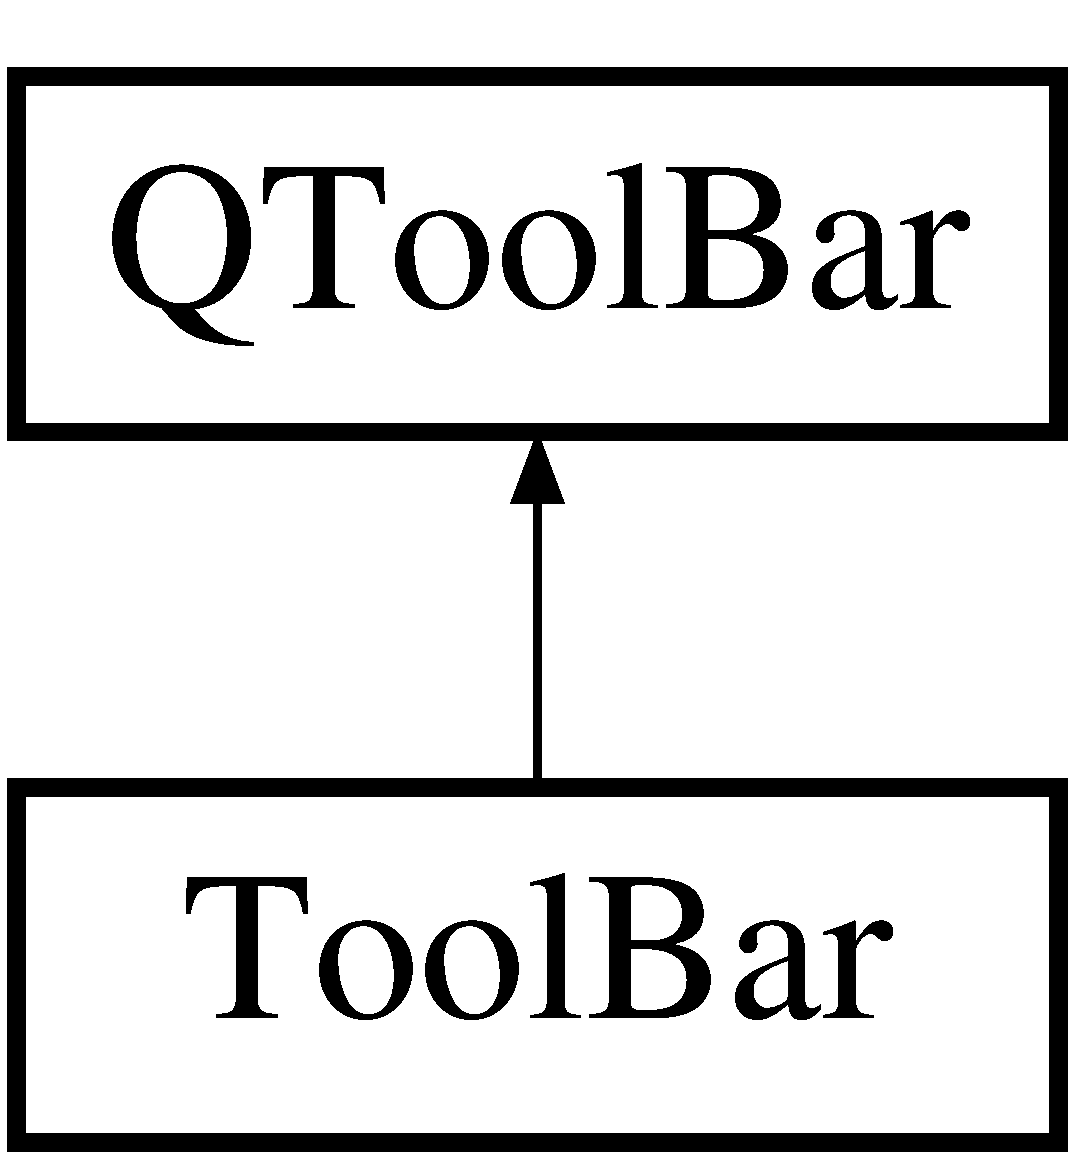
\includegraphics[height=2.000000cm]{class_tool_bar}
\end{center}
\end{figure}
\subsection*{Public Member Functions}
\begin{DoxyCompactItemize}
\item 
\hypertarget{class_tool_bar_a8cc37599b68c6b40d508ffb6b37ebcac}{{\bfseries Tool\-Bar} (const Q\-String \&title, Q\-Widget $\ast$parent)}\label{class_tool_bar_a8cc37599b68c6b40d508ffb6b37ebcac}

\end{DoxyCompactItemize}
\subsection*{Public Attributes}
\begin{DoxyCompactItemize}
\item 
\hypertarget{class_tool_bar_a41a552950d88c7ddf220ec9443ca7555}{Q\-Menu $\ast$ {\bfseries menu}}\label{class_tool_bar_a41a552950d88c7ddf220ec9443ca7555}

\end{DoxyCompactItemize}
\subsection*{Protected Member Functions}
\begin{DoxyCompactItemize}
\item 
\hypertarget{class_tool_bar_a9f936f5a0e51703c9163c4f4ca43b803}{void {\bfseries enter\-Event} (Q\-Event $\ast$)}\label{class_tool_bar_a9f936f5a0e51703c9163c4f4ca43b803}

\item 
\hypertarget{class_tool_bar_a3a4176e2c929e7d0fdd6431d62e3ae0d}{void {\bfseries leave\-Event} (Q\-Event $\ast$)}\label{class_tool_bar_a3a4176e2c929e7d0fdd6431d62e3ae0d}

\end{DoxyCompactItemize}


The documentation for this class was generated from the following files\-:\begin{DoxyCompactItemize}
\item 
toolbar.\-h\item 
toolbar.\-cpp\end{DoxyCompactItemize}

\hypertarget{class_tool_box}{\section{Tool\-Box Class Reference}
\label{class_tool_box}\index{Tool\-Box@{Tool\-Box}}
}
Inheritance diagram for Tool\-Box\-:\begin{figure}[H]
\begin{center}
\leavevmode
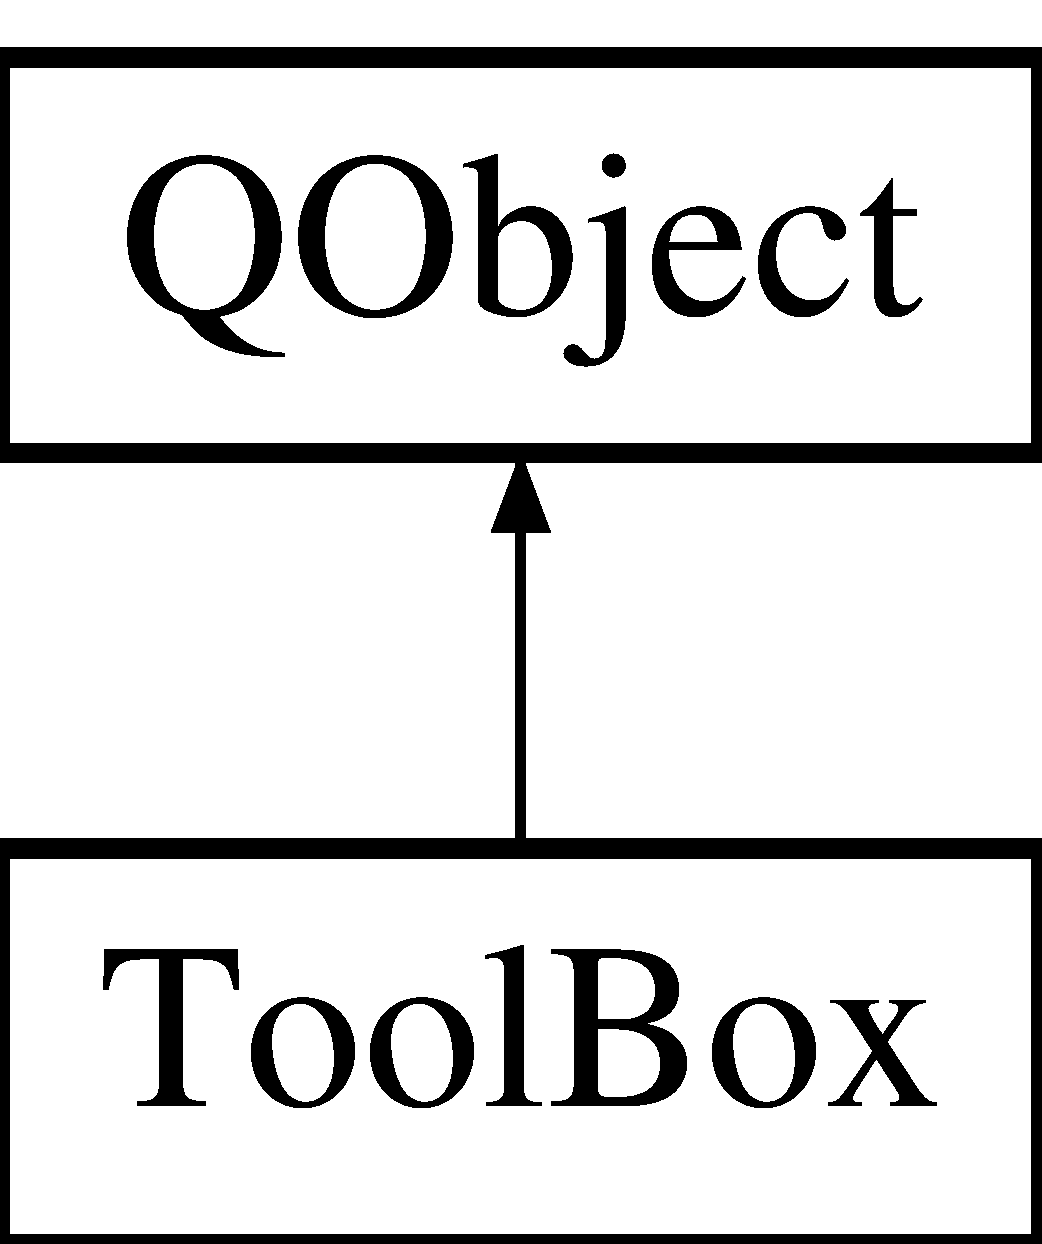
\includegraphics[height=2.000000cm]{class_tool_box}
\end{center}
\end{figure}
\subsection*{Public Member Functions}
\begin{DoxyCompactItemize}
\item 
\hypertarget{class_tool_box_a7849f505611d7b236c2e3cd548fd8a16}{{\bfseries Tool\-Box} (Q\-Widget $\ast$parent)}\label{class_tool_box_a7849f505611d7b236c2e3cd548fd8a16}

\end{DoxyCompactItemize}
\subsection*{Public Attributes}
\begin{DoxyCompactItemize}
\item 
\hypertarget{class_tool_box_a7490ce2cf614dc111418017c693fa2b6}{Q\-List$<$ Q\-Tool\-Bar $\ast$ $>$ {\bfseries tool\-Bar\-List}}\label{class_tool_box_a7490ce2cf614dc111418017c693fa2b6}

\item 
\hypertarget{class_tool_box_a188312362e14384284a1afcbe9248b05}{Q\-Tool\-Bar $\ast$ {\bfseries current\-Tool\-Bar}}\label{class_tool_box_a188312362e14384284a1afcbe9248b05}

\item 
\hypertarget{class_tool_box_af98b33face328ff6577748bdc1fda5de}{Q\-Tool\-Bar $\ast$ {\bfseries marquee\-Tool\-Bar}}\label{class_tool_box_af98b33face328ff6577748bdc1fda5de}

\item 
\hypertarget{class_tool_box_a8b2c3b4f8a7af99c0e0a1780e7edc03a}{Q\-Tool\-Bar $\ast$ {\bfseries brush\-Tool\-Bar}}\label{class_tool_box_a8b2c3b4f8a7af99c0e0a1780e7edc03a}

\item 
\hypertarget{class_tool_box_ae06fd23deb77253946ded679850071a9}{Q\-Tool\-Bar $\ast$ {\bfseries pen\-Tool\-Bar}}\label{class_tool_box_ae06fd23deb77253946ded679850071a9}

\item 
\hypertarget{class_tool_box_a6de2469d94a1598bb97c754937e133e7}{Q\-Spin\-Box $\ast$ {\bfseries pen\-Size}}\label{class_tool_box_a6de2469d94a1598bb97c754937e133e7}

\end{DoxyCompactItemize}


The documentation for this class was generated from the following files\-:\begin{DoxyCompactItemize}
\item 
toolbox.\-h\item 
toolbox.\-cpp\end{DoxyCompactItemize}

\hypertarget{class_tool_tweak}{\section{Tool\-Tweak Class Reference}
\label{class_tool_tweak}\index{Tool\-Tweak@{Tool\-Tweak}}
}
Inheritance diagram for Tool\-Tweak\-:\begin{figure}[H]
\begin{center}
\leavevmode
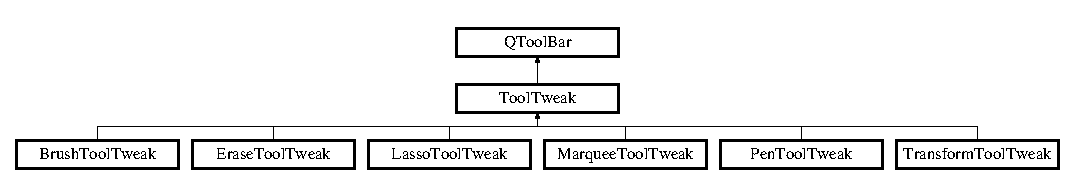
\includegraphics[height=2.043796cm]{class_tool_tweak}
\end{center}
\end{figure}
\subsection*{Public Member Functions}
\begin{DoxyCompactItemize}
\item 
\hypertarget{class_tool_tweak_abb2e54f714e34704f6b02dc2d1033634}{{\bfseries Tool\-Tweak} (const Q\-String \&title, Q\-Widget $\ast$parent)}\label{class_tool_tweak_abb2e54f714e34704f6b02dc2d1033634}

\end{DoxyCompactItemize}


The documentation for this class was generated from the following files\-:\begin{DoxyCompactItemize}
\item 
toolbox.\-h\item 
toolbox.\-cpp\end{DoxyCompactItemize}

\hypertarget{class_tool_type}{\section{Tool\-Type Class Reference}
\label{class_tool_type}\index{Tool\-Type@{Tool\-Type}}
}
\subsection*{Public Types}
\begin{DoxyCompactItemize}
\item 
enum {\bfseries tool\-Type} \{ \\*
{\bfseries Brush} =0, 
{\bfseries Erase} =1, 
{\bfseries Marquee} =2, 
{\bfseries Pen} =3, 
\\*
{\bfseries Transform} =4, 
{\bfseries Lasso} =5
 \}
\end{DoxyCompactItemize}


The documentation for this class was generated from the following file\-:\begin{DoxyCompactItemize}
\item 
toolbox.\-h\end{DoxyCompactItemize}

\hypertarget{class_transform_tool_base}{\section{Transform\-Tool\-Base Class Reference}
\label{class_transform_tool_base}\index{Transform\-Tool\-Base@{Transform\-Tool\-Base}}
}
Inheritance diagram for Transform\-Tool\-Base\-:\begin{figure}[H]
\begin{center}
\leavevmode
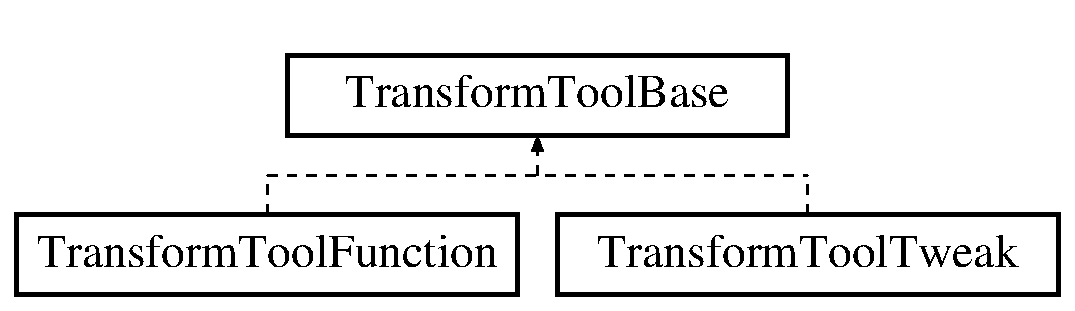
\includegraphics[height=2.000000cm]{class_transform_tool_base}
\end{center}
\end{figure}


The documentation for this class was generated from the following file\-:\begin{DoxyCompactItemize}
\item 
toolbox.\-h\end{DoxyCompactItemize}

\hypertarget{class_transform_tool_function}{\section{Transform\-Tool\-Function Class Reference}
\label{class_transform_tool_function}\index{Transform\-Tool\-Function@{Transform\-Tool\-Function}}
}
Inheritance diagram for Transform\-Tool\-Function\-:\begin{figure}[H]
\begin{center}
\leavevmode
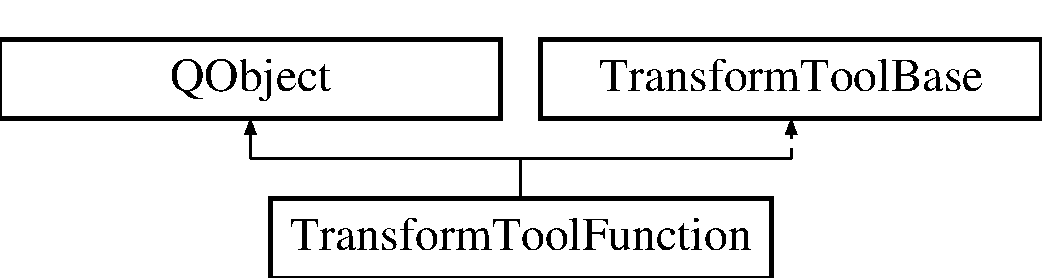
\includegraphics[height=2.000000cm]{class_transform_tool_function}
\end{center}
\end{figure}
\subsection*{Public Member Functions}
\begin{DoxyCompactItemize}
\item 
\hypertarget{class_transform_tool_function_a03cfa9a4e1da1303959f9da434de0ab5}{{\bfseries Transform\-Tool\-Function} (Q\-Widget $\ast$parent)}\label{class_transform_tool_function_a03cfa9a4e1da1303959f9da434de0ab5}

\end{DoxyCompactItemize}


The documentation for this class was generated from the following files\-:\begin{DoxyCompactItemize}
\item 
toolbox.\-h\item 
toolbox.\-cpp\end{DoxyCompactItemize}

\hypertarget{class_transform_tool_tweak}{\section{Transform\-Tool\-Tweak Class Reference}
\label{class_transform_tool_tweak}\index{Transform\-Tool\-Tweak@{Transform\-Tool\-Tweak}}
}
Inheritance diagram for Transform\-Tool\-Tweak\-:\begin{figure}[H]
\begin{center}
\leavevmode
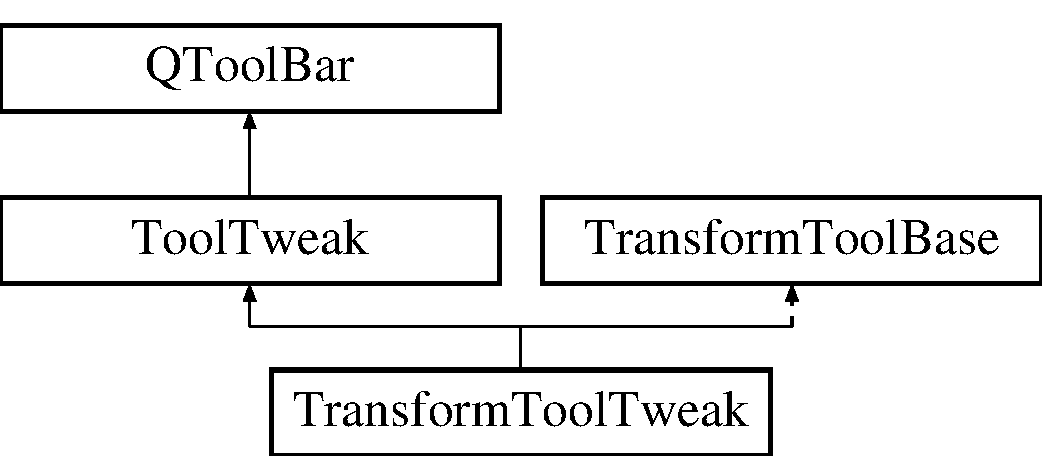
\includegraphics[height=3.000000cm]{class_transform_tool_tweak}
\end{center}
\end{figure}
\subsection*{Public Member Functions}
\begin{DoxyCompactItemize}
\item 
\hypertarget{class_transform_tool_tweak_afc1a7633c591d1eb0b1ebcf912857060}{{\bfseries Transform\-Tool\-Tweak} (Q\-Widget $\ast$parent)}\label{class_transform_tool_tweak_afc1a7633c591d1eb0b1ebcf912857060}

\end{DoxyCompactItemize}


The documentation for this class was generated from the following files\-:\begin{DoxyCompactItemize}
\item 
toolbox.\-h\item 
toolbox.\-cpp\end{DoxyCompactItemize}

%--- End generated contents ---

% Index
\newpage
\phantomsection
\addcontentsline{toc}{part}{Index}
\printindex

\end{document}
